\section{Diâmetro}

\begin{frame}[fragile]{Diâmetro de uma árvore}

    \begin{itemize}
        \item O diâmetro de uma árvore é igual ao maior dentre todos os tamanhos dos caminhos
            entre os pares de vértices $u$ e $v$ do grafo

        \item O maior caminho que produz o diâmetro não é, necessariamente, único

        \item Computar estas distâncias utilizando o algoritmo de Floyd-Warshall em $O(V^3)$ e,
            em seguida, determinar a maior dentre estas distâncias em $O(V^2$) produziria
            o resultado correto

        \item Porém é possível chegar ao mesmo resultado de duas maneiras: com programação
            dinâmica ou com duas DFS

        \item Em ambos casos, a complexidade é $O(V)$

    \end{itemize}

\end{frame}

\begin{frame}[fragile]{Visualização do diâmetro de uma árvore}

    \begin{tikzpicture}

        \begin{scope}{shift={(3,0)}}
            \node[opacity=0] (X) at (-1.5, 0) { $1$ };
            \node[circle,draw] (A) at (0, 0) { $1$ };
            \node[circle,draw] (B) at (0, 4) { $3$ };
            \node[circle,draw] (C) at (2, 2) { $7$ };
            \node[circle,draw] (D) at (4, 3) { $4$ };
            \node[circle,draw] (E) at (4, 1) { $2$ };
            \node[circle,draw] (F) at (6, 5) { $5$ };
            \node[circle,draw] (G) at (7, 2) { $6$ };

            \draw[ultra thick] (A) -- (C);
            \draw (B) -- (C);
            \draw[ultra thick] (C) -- (D);
            \draw (D) -- (E);
            \draw[ultra thick] (D) -- (F);
            \draw[ultra thick] (F) -- (G);

            \node at (0, 6) { Diâmetro: 4 };
        \end{scope}
    \end{tikzpicture}

\end{frame}

\begin{frame}[fragile]{Diâmetro com programação dinâmica}

    \begin{itemize}
        \item Para computar o diâmetro com programação dinâmica é preciso observar que, em
            uma árvore com raiz, cada caminho possui um pico: o nó que está posicionado no nível
            mais alto da árvore

        \item Assim, para cada nó $u$ da árvore, será computado \code{c}{max_length[u]}: o tamanho
            do maior caminho que tem $u$ como pico

        \item Dentre todos estes caminhos, um deles fornecerá o diâmetro

        \item Para computar \code{c}{max_length[u]}, basta recorrer à rotina que computa
            \code{c}{to_leaf[v]} para todos os filhos $v$ de $u$

        \item Se $u$ não tem filhos, \code{c}{max_length[u]} = 0
        \item Se $u$ tem apenas um filho, \code{c}{max_length[u]} = \code{c}{to_leaf[v]} + 1
        \item Se $u$ tem dois ou mais filhos, \code{c}{max_length[u]} = \code{c}{to_leaf[v]} + 
            \code{c}{to_leaf[w]} + 2, onde $v$ e $w$ são dois filhos distintos com os maiores
            valores \code{c}{to_leaf} dentre todos os filhos de $u$

    \end{itemize}

\end{frame}

\begin{frame}[fragile]{Visualização do algoritmo que computa o diâmetro com DP}

    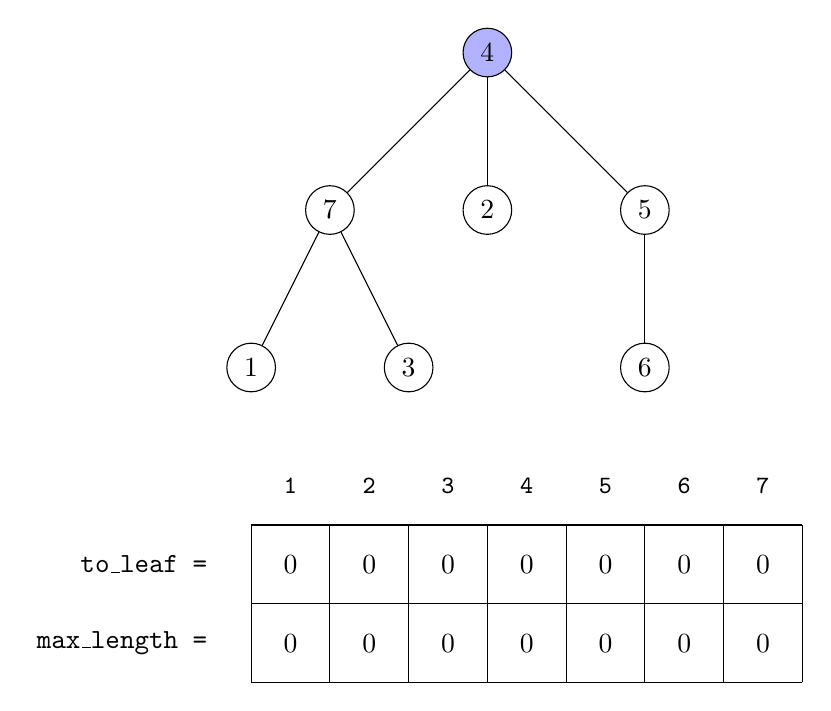
\begin{tikzpicture}

        \begin{scope}
            %\node[opacity=0] (X) at (-1, 0) { $1$ };

            \node[fill=blue!30,circle,draw] (D) at (4, 5) { $4$ };
            \node[circle,draw] (C) at (2, 3) { $7$ };
            \node[circle,draw,fill=white!30] (E) at (4, 3) { $2$ };
            \node[circle,draw] (F) at (6, 3) { $5$ };
            \node[circle,draw,fill=white!30] (A) at (1, 1) { $1$ };
            \node[circle,draw,fill=white!30] (B) at (3, 1) { $3$ };
            \node[circle,draw,fill=white!30] (G) at (6, 1) { $6$ };

            \draw (A) -- (C);
            \draw (B) -- (C);
            \draw (C) -- (D);
            \draw (D) -- (E);
            \draw (D) -- (F);
            \draw (F) -- (G);

            \node[anchor=east] at (0.75, -1.5) { \texttt{to\_leaf = } };
            \draw (1, -2) grid (8, -1);

            \node[anchor=east] at (0.75, -2.5) { \texttt{max\_length = } };
            \draw (1, -3) grid (8, -2);

            \node at (1.5, -0.5) { \small \texttt{1} };
            \node at (2.5, -0.5) { \small \texttt{2} };
            \node at (3.5, -0.5) { \small \texttt{3} };
            \node at (4.5, -0.5) { \small \texttt{4} };
            \node at (5.5, -0.5) { \small \texttt{5} };
            \node at (6.5, -0.5) { \small \texttt{6} };
            \node at (7.5, -0.5) { \small \texttt{7} };

            \node at (1.5, -1.5) { $0$ };
            \node at (2.5, -1.5) { $0$ };
            \node at (3.5, -1.5) { $0$ };
            \node at (4.5, -1.5) { \textcolor{black}{$0$} };
            \node at (5.5, -1.5) { $0$ };
            \node at (6.5, -1.5) { $0$ };
            \node at (7.5, -1.5) { $0$ };

            \node at (1.5, -2.5) { $0$ };
            \node at (2.5, -2.5) { $0$ };
            \node at (3.5, -2.5) { $0$ };
            \node at (4.5, -2.5) { \textcolor{black}{$0$} };
            \node at (5.5, -2.5) { $0$ };
            \node at (6.5, -2.5) { $0$ };
            \node at (7.5, -2.5) { $0$ };


        \end{scope}
    \end{tikzpicture}

\end{frame}

\begin{frame}[fragile]{Visualização do algoritmo que computa o diâmetro com DP}

    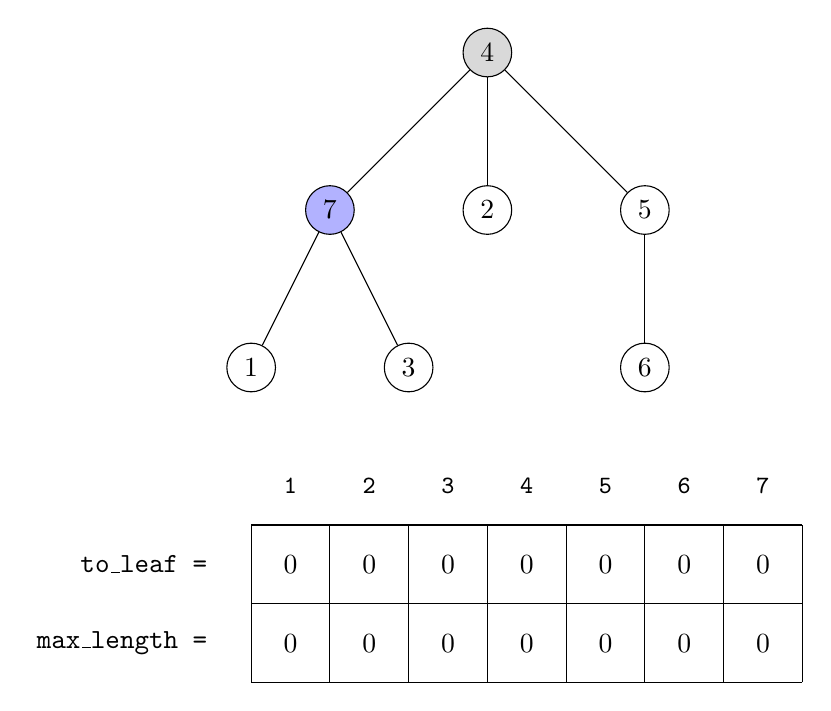
\begin{tikzpicture}

        \begin{scope}
            %\node[opacity=0] (X) at (-1, 0) { $1$ };

            \node[fill=gray!30,circle,draw] (D) at (4, 5) { $4$ };
            \node[circle,draw,fill=blue!30] (C) at (2, 3) { $7$ };
            \node[circle,draw,fill=white!30] (E) at (4, 3) { $2$ };
            \node[circle,draw] (F) at (6, 3) { $5$ };
            \node[circle,draw,fill=white!30] (A) at (1, 1) { $1$ };
            \node[circle,draw,fill=white!30] (B) at (3, 1) { $3$ };
            \node[circle,draw,fill=white!30] (G) at (6, 1) { $6$ };

            \draw (A) -- (C);
            \draw (B) -- (C);
            \draw (C) -- (D);
            \draw (D) -- (E);
            \draw (D) -- (F);
            \draw (F) -- (G);

            \node[anchor=east] at (0.75, -1.5) { \texttt{to\_leaf = } };
            \draw (1, -2) grid (8, -1);

            \node[anchor=east] at (0.75, -2.5) { \texttt{max\_length = } };
            \draw (1, -3) grid (8, -2);

            \node at (1.5, -0.5) { \small \texttt{1} };
            \node at (2.5, -0.5) { \small \texttt{2} };
            \node at (3.5, -0.5) { \small \texttt{3} };
            \node at (4.5, -0.5) { \small \texttt{4} };
            \node at (5.5, -0.5) { \small \texttt{5} };
            \node at (6.5, -0.5) { \small \texttt{6} };
            \node at (7.5, -0.5) { \small \texttt{7} };

            \node at (1.5, -1.5) { $0$ };
            \node at (2.5, -1.5) { $0$ };
            \node at (3.5, -1.5) { $0$ };
            \node at (4.5, -1.5) { \textcolor{black}{$0$} };
            \node at (5.5, -1.5) { $0$ };
            \node at (6.5, -1.5) { $0$ };
            \node at (7.5, -1.5) { $0$ };

            \node at (1.5, -2.5) { $0$ };
            \node at (2.5, -2.5) { $0$ };
            \node at (3.5, -2.5) { $0$ };
            \node at (4.5, -2.5) { \textcolor{black}{$0$} };
            \node at (5.5, -2.5) { $0$ };
            \node at (6.5, -2.5) { $0$ };
            \node at (7.5, -2.5) { $0$ };


        \end{scope}
    \end{tikzpicture}

\end{frame}

\begin{frame}[fragile]{Visualização do algoritmo que computa o diâmetro com DP}

    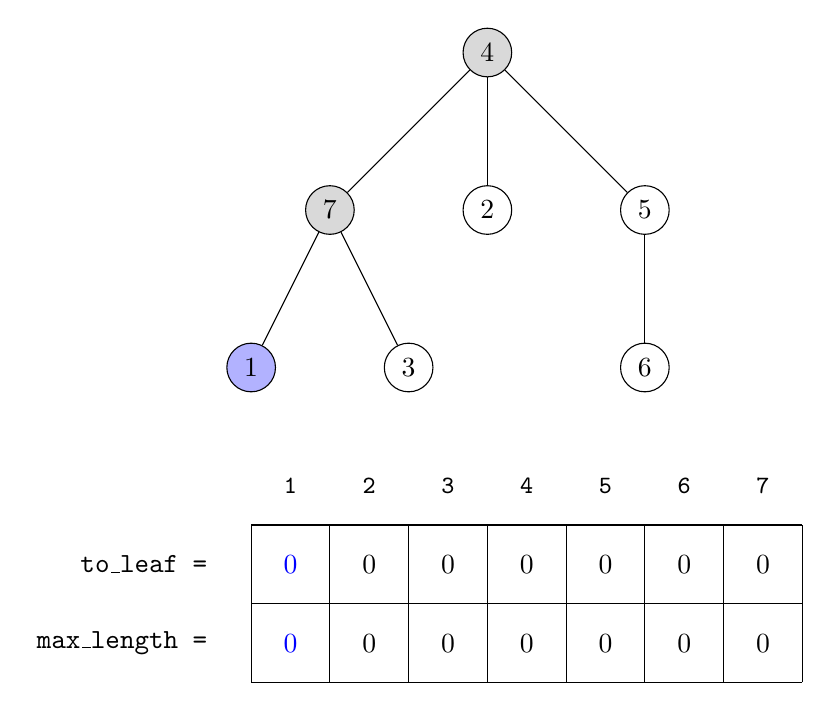
\begin{tikzpicture}

        \begin{scope}
            %\node[opacity=0] (X) at (-1, 0) { $1$ };

            \node[fill=gray!30,circle,draw] (D) at (4, 5) { $4$ };
            \node[circle,draw,fill=gray!30] (C) at (2, 3) { $7$ };
            \node[circle,draw,fill=white!30] (E) at (4, 3) { $2$ };
            \node[circle,draw] (F) at (6, 3) { $5$ };
            \node[circle,draw,fill=blue!30] (A) at (1, 1) { $1$ };
            \node[circle,draw,fill=white!30] (B) at (3, 1) { $3$ };
            \node[circle,draw,fill=white!30] (G) at (6, 1) { $6$ };

            \draw (A) -- (C);
            \draw (B) -- (C);
            \draw (C) -- (D);
            \draw (D) -- (E);
            \draw (D) -- (F);
            \draw (F) -- (G);

            \node[anchor=east] at (0.75, -1.5) { \texttt{to\_leaf = } };
            \draw (1, -2) grid (8, -1);

            \node[anchor=east] at (0.75, -2.5) { \texttt{max\_length = } };
            \draw (1, -3) grid (8, -2);

            \node at (1.5, -0.5) { \small \texttt{1} };
            \node at (2.5, -0.5) { \small \texttt{2} };
            \node at (3.5, -0.5) { \small \texttt{3} };
            \node at (4.5, -0.5) { \small \texttt{4} };
            \node at (5.5, -0.5) { \small \texttt{5} };
            \node at (6.5, -0.5) { \small \texttt{6} };
            \node at (7.5, -0.5) { \small \texttt{7} };

            \node at (1.5, -1.5) { \textcolor{blue}{$0$} };
            \node at (2.5, -1.5) { $0$ };
            \node at (3.5, -1.5) { $0$ };
            \node at (4.5, -1.5) { \textcolor{black}{$0$} };
            \node at (5.5, -1.5) { $0$ };
            \node at (6.5, -1.5) { $0$ };
            \node at (7.5, -1.5) { $0$ };

            \node at (1.5, -2.5) { \textcolor{blue}{$0$} };
            \node at (2.5, -2.5) { $0$ };
            \node at (3.5, -2.5) { $0$ };
            \node at (4.5, -2.5) { \textcolor{black}{$0$} };
            \node at (5.5, -2.5) { $0$ };
            \node at (6.5, -2.5) { $0$ };
            \node at (7.5, -2.5) { $0$ };


        \end{scope}
    \end{tikzpicture}

\end{frame}

\begin{frame}[fragile]{Visualização do algoritmo que computa o diâmetro com DP}

    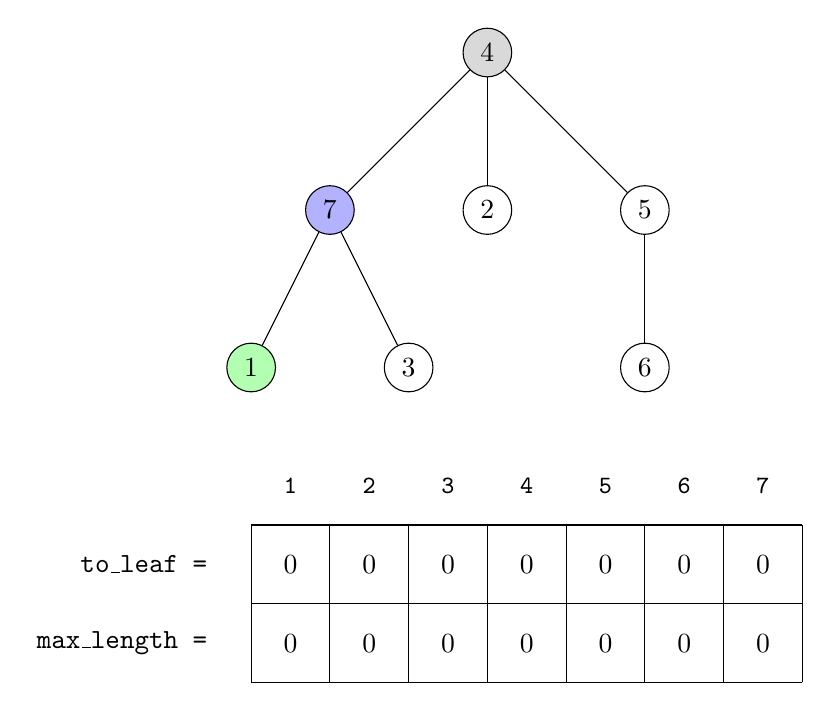
\begin{tikzpicture}

        \begin{scope}
            %\node[opacity=0] (X) at (-1, 0) { $1$ };

            \node[fill=gray!30,circle,draw] (D) at (4, 5) { $4$ };
            \node[circle,draw,fill=blue!30] (C) at (2, 3) { $7$ };
            \node[circle,draw,fill=white!30] (E) at (4, 3) { $2$ };
            \node[circle,draw] (F) at (6, 3) { $5$ };
            \node[circle,draw,fill=green!30] (A) at (1, 1) { $1$ };
            \node[circle,draw,fill=white!30] (B) at (3, 1) { $3$ };
            \node[circle,draw,fill=white!30] (G) at (6, 1) { $6$ };

            \draw (A) -- (C);
            \draw (B) -- (C);
            \draw (C) -- (D);
            \draw (D) -- (E);
            \draw (D) -- (F);
            \draw (F) -- (G);

            \node[anchor=east] at (0.75, -1.5) { \texttt{to\_leaf = } };
            \draw (1, -2) grid (8, -1);

            \node[anchor=east] at (0.75, -2.5) { \texttt{max\_length = } };
            \draw (1, -3) grid (8, -2);

            \node at (1.5, -0.5) { \small \texttt{1} };
            \node at (2.5, -0.5) { \small \texttt{2} };
            \node at (3.5, -0.5) { \small \texttt{3} };
            \node at (4.5, -0.5) { \small \texttt{4} };
            \node at (5.5, -0.5) { \small \texttt{5} };
            \node at (6.5, -0.5) { \small \texttt{6} };
            \node at (7.5, -0.5) { \small \texttt{7} };

            \node at (1.5, -1.5) { \textcolor{black}{$0$} };
            \node at (2.5, -1.5) { $0$ };
            \node at (3.5, -1.5) { $0$ };
            \node at (4.5, -1.5) { \textcolor{black}{$0$} };
            \node at (5.5, -1.5) { $0$ };
            \node at (6.5, -1.5) { $0$ };
            \node at (7.5, -1.5) { $0$ };

            \node at (1.5, -2.5) { \textcolor{black}{$0$} };
            \node at (2.5, -2.5) { $0$ };
            \node at (3.5, -2.5) { $0$ };
            \node at (4.5, -2.5) { \textcolor{black}{$0$} };
            \node at (5.5, -2.5) { $0$ };
            \node at (6.5, -2.5) { $0$ };
            \node at (7.5, -2.5) { $0$ };


        \end{scope}
    \end{tikzpicture}

\end{frame}

\begin{frame}[fragile]{Visualização do algoritmo que computa o diâmetro com DP}

    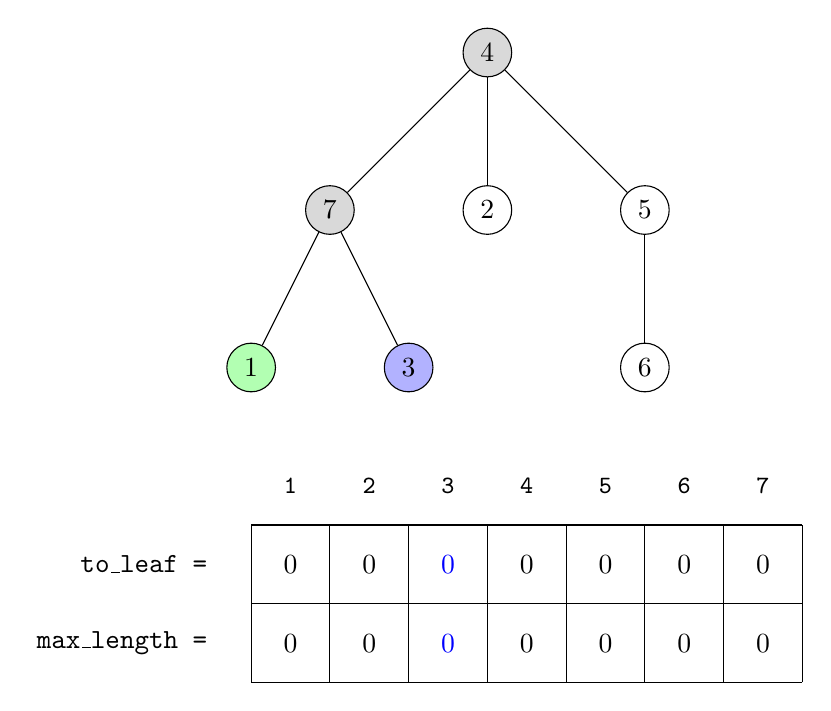
\begin{tikzpicture}

        \begin{scope}
            %\node[opacity=0] (X) at (-1, 0) { $1$ };

            \node[fill=gray!30,circle,draw] (D) at (4, 5) { $4$ };
            \node[circle,draw,fill=gray!30] (C) at (2, 3) { $7$ };
            \node[circle,draw,fill=white!30] (E) at (4, 3) { $2$ };
            \node[circle,draw] (F) at (6, 3) { $5$ };
            \node[circle,draw,fill=green!30] (A) at (1, 1) { $1$ };
            \node[circle,draw,fill=blue!30] (B) at (3, 1) { $3$ };
            \node[circle,draw,fill=white!30] (G) at (6, 1) { $6$ };

            \draw (A) -- (C);
            \draw (B) -- (C);
            \draw (C) -- (D);
            \draw (D) -- (E);
            \draw (D) -- (F);
            \draw (F) -- (G);

            \node[anchor=east] at (0.75, -1.5) { \texttt{to\_leaf = } };
            \draw (1, -2) grid (8, -1);

            \node[anchor=east] at (0.75, -2.5) { \texttt{max\_length = } };
            \draw (1, -3) grid (8, -2);

            \node at (1.5, -0.5) { \small \texttt{1} };
            \node at (2.5, -0.5) { \small \texttt{2} };
            \node at (3.5, -0.5) { \small \texttt{3} };
            \node at (4.5, -0.5) { \small \texttt{4} };
            \node at (5.5, -0.5) { \small \texttt{5} };
            \node at (6.5, -0.5) { \small \texttt{6} };
            \node at (7.5, -0.5) { \small \texttt{7} };

            \node at (1.5, -1.5) { \textcolor{black}{$0$} };
            \node at (2.5, -1.5) { $0$ };
            \node at (3.5, -1.5) { \textcolor{blue}{$0$} };
            \node at (4.5, -1.5) { \textcolor{black}{$0$} };
            \node at (5.5, -1.5) { $0$ };
            \node at (6.5, -1.5) { $0$ };
            \node at (7.5, -1.5) { $0$ };

            \node at (1.5, -2.5) { \textcolor{black}{$0$} };
            \node at (2.5, -2.5) { $0$ };
            \node at (3.5, -2.5) { \textcolor{blue}{$0$} };
            \node at (4.5, -2.5) { \textcolor{black}{$0$} };
            \node at (5.5, -2.5) { $0$ };
            \node at (6.5, -2.5) { $0$ };
            \node at (7.5, -2.5) { $0$ };


        \end{scope}
    \end{tikzpicture}

\end{frame}

\begin{frame}[fragile]{Visualização do algoritmo que computa o diâmetro com DP}

    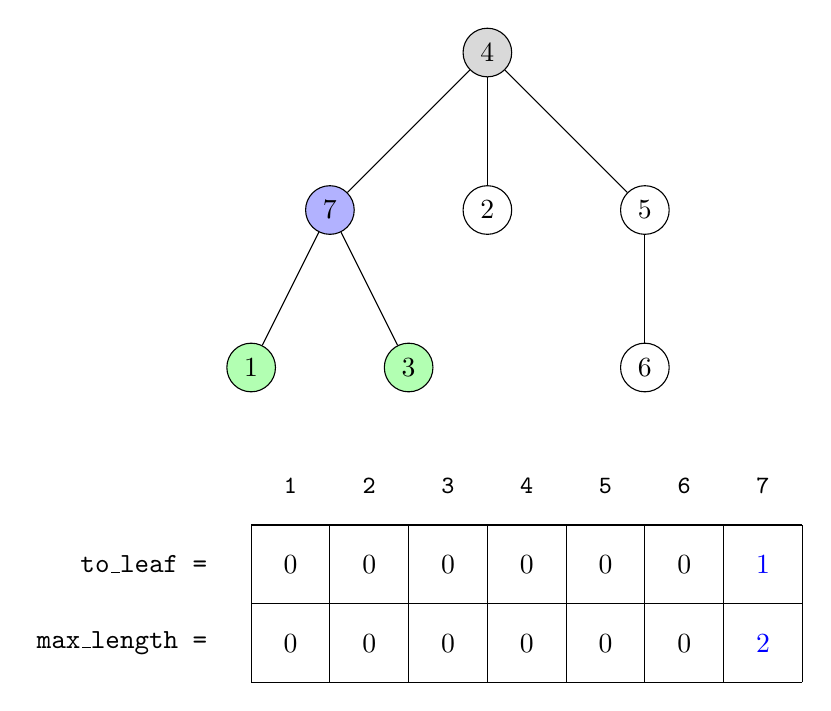
\begin{tikzpicture}

        \begin{scope}
            %\node[opacity=0] (X) at (-1, 0) { $1$ };

            \node[fill=gray!30,circle,draw] (D) at (4, 5) { $4$ };
            \node[circle,draw,fill=blue!30] (C) at (2, 3) { $7$ };
            \node[circle,draw,fill=white!30] (E) at (4, 3) { $2$ };
            \node[circle,draw] (F) at (6, 3) { $5$ };
            \node[circle,draw,fill=green!30] (A) at (1, 1) { $1$ };
            \node[circle,draw,fill=green!30] (B) at (3, 1) { $3$ };
            \node[circle,draw,fill=white!30] (G) at (6, 1) { $6$ };

            \draw (A) -- (C);
            \draw (B) -- (C);
            \draw (C) -- (D);
            \draw (D) -- (E);
            \draw (D) -- (F);
            \draw (F) -- (G);

            \node[anchor=east] at (0.75, -1.5) { \texttt{to\_leaf = } };
            \draw (1, -2) grid (8, -1);

            \node[anchor=east] at (0.75, -2.5) { \texttt{max\_length = } };
            \draw (1, -3) grid (8, -2);

            \node at (1.5, -0.5) { \small \texttt{1} };
            \node at (2.5, -0.5) { \small \texttt{2} };
            \node at (3.5, -0.5) { \small \texttt{3} };
            \node at (4.5, -0.5) { \small \texttt{4} };
            \node at (5.5, -0.5) { \small \texttt{5} };
            \node at (6.5, -0.5) { \small \texttt{6} };
            \node at (7.5, -0.5) { \small \texttt{7} };

            \node at (1.5, -1.5) { \textcolor{black}{$0$} };
            \node at (2.5, -1.5) { $0$ };
            \node at (3.5, -1.5) { \textcolor{black}{$0$} };
            \node at (4.5, -1.5) { \textcolor{black}{$0$} };
            \node at (5.5, -1.5) { $0$ };
            \node at (6.5, -1.5) { $0$ };
            \node at (7.5, -1.5) { \textcolor{blue}{$1$} };

            \node at (1.5, -2.5) { \textcolor{black}{$0$} };
            \node at (2.5, -2.5) { $0$ };
            \node at (3.5, -2.5) { \textcolor{black}{$0$} };
            \node at (4.5, -2.5) { \textcolor{black}{$0$} };
            \node at (5.5, -2.5) { $0$ };
            \node at (6.5, -2.5) { $0$ };
            \node at (7.5, -2.5) { \textcolor{blue}{$2$} };


        \end{scope}
    \end{tikzpicture}

\end{frame}

\begin{frame}[fragile]{Visualização do algoritmo que computa o diâmetro com DP}

    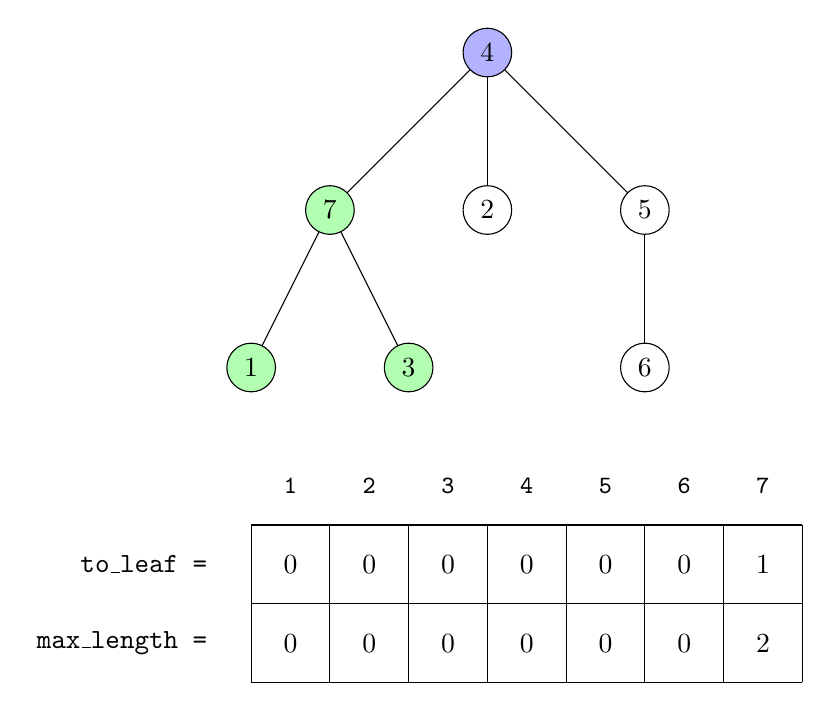
\begin{tikzpicture}

        \begin{scope}
            %\node[opacity=0] (X) at (-1, 0) { $1$ };

            \node[fill=blue!30,circle,draw] (D) at (4, 5) { $4$ };
            \node[circle,draw,fill=green!30] (C) at (2, 3) { $7$ };
            \node[circle,draw,fill=white!30] (E) at (4, 3) { $2$ };
            \node[circle,draw] (F) at (6, 3) { $5$ };
            \node[circle,draw,fill=green!30] (A) at (1, 1) { $1$ };
            \node[circle,draw,fill=green!30] (B) at (3, 1) { $3$ };
            \node[circle,draw,fill=white!30] (G) at (6, 1) { $6$ };

            \draw (A) -- (C);
            \draw (B) -- (C);
            \draw (C) -- (D);
            \draw (D) -- (E);
            \draw (D) -- (F);
            \draw (F) -- (G);

            \node[anchor=east] at (0.75, -1.5) { \texttt{to\_leaf = } };
            \draw (1, -2) grid (8, -1);

            \node[anchor=east] at (0.75, -2.5) { \texttt{max\_length = } };
            \draw (1, -3) grid (8, -2);

            \node at (1.5, -0.5) { \small \texttt{1} };
            \node at (2.5, -0.5) { \small \texttt{2} };
            \node at (3.5, -0.5) { \small \texttt{3} };
            \node at (4.5, -0.5) { \small \texttt{4} };
            \node at (5.5, -0.5) { \small \texttt{5} };
            \node at (6.5, -0.5) { \small \texttt{6} };
            \node at (7.5, -0.5) { \small \texttt{7} };

            \node at (1.5, -1.5) { \textcolor{black}{$0$} };
            \node at (2.5, -1.5) { $0$ };
            \node at (3.5, -1.5) { \textcolor{black}{$0$} };
            \node at (4.5, -1.5) { \textcolor{black}{$0$} };
            \node at (5.5, -1.5) { $0$ };
            \node at (6.5, -1.5) { $0$ };
            \node at (7.5, -1.5) { \textcolor{black}{$1$} };

            \node at (1.5, -2.5) { \textcolor{black}{$0$} };
            \node at (2.5, -2.5) { $0$ };
            \node at (3.5, -2.5) { \textcolor{black}{$0$} };
            \node at (4.5, -2.5) { \textcolor{black}{$0$} };
            \node at (5.5, -2.5) { $0$ };
            \node at (6.5, -2.5) { $0$ };
            \node at (7.5, -2.5) { \textcolor{black}{$2$} };


        \end{scope}
    \end{tikzpicture}

\end{frame}

\begin{frame}[fragile]{Visualização do algoritmo que computa o diâmetro com DP}

    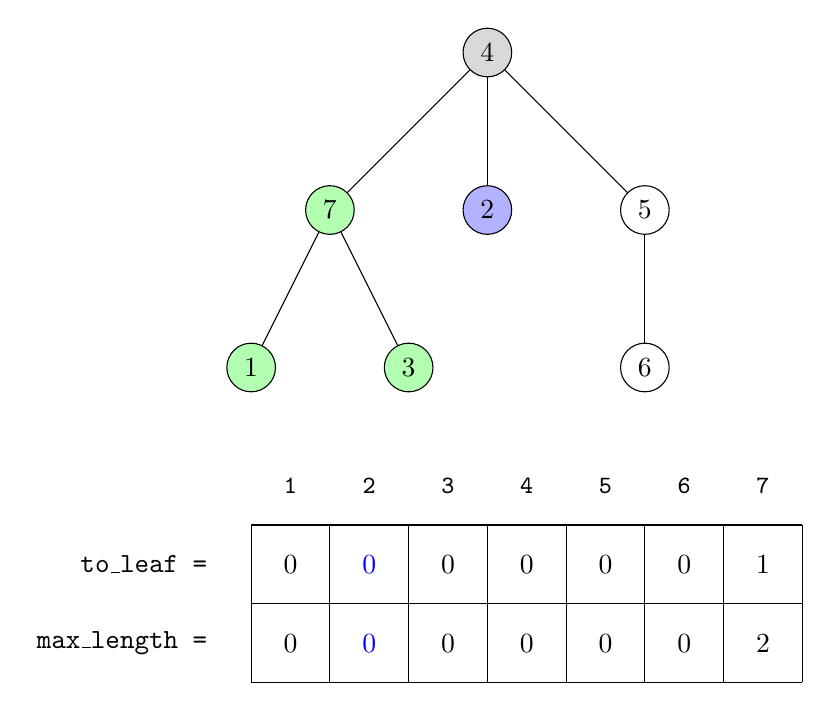
\begin{tikzpicture}

        \begin{scope}
            %\node[opacity=0] (X) at (-1, 0) { $1$ };

            \node[fill=gray!30,circle,draw] (D) at (4, 5) { $4$ };
            \node[circle,draw,fill=green!30] (C) at (2, 3) { $7$ };
            \node[circle,draw,fill=blue!30] (E) at (4, 3) { $2$ };
            \node[circle,draw] (F) at (6, 3) { $5$ };
            \node[circle,draw,fill=green!30] (A) at (1, 1) { $1$ };
            \node[circle,draw,fill=green!30] (B) at (3, 1) { $3$ };
            \node[circle,draw,fill=white!30] (G) at (6, 1) { $6$ };

            \draw (A) -- (C);
            \draw (B) -- (C);
            \draw (C) -- (D);
            \draw (D) -- (E);
            \draw (D) -- (F);
            \draw (F) -- (G);

            \node[anchor=east] at (0.75, -1.5) { \texttt{to\_leaf = } };
            \draw (1, -2) grid (8, -1);

            \node[anchor=east] at (0.75, -2.5) { \texttt{max\_length = } };
            \draw (1, -3) grid (8, -2);

            \node at (1.5, -0.5) { \small \texttt{1} };
            \node at (2.5, -0.5) { \small \texttt{2} };
            \node at (3.5, -0.5) { \small \texttt{3} };
            \node at (4.5, -0.5) { \small \texttt{4} };
            \node at (5.5, -0.5) { \small \texttt{5} };
            \node at (6.5, -0.5) { \small \texttt{6} };
            \node at (7.5, -0.5) { \small \texttt{7} };

            \node at (1.5, -1.5) { \textcolor{black}{$0$} };
            \node at (2.5, -1.5) { \textcolor{blue}{$0$} };
            \node at (3.5, -1.5) { \textcolor{black}{$0$} };
            \node at (4.5, -1.5) { \textcolor{black}{$0$} };
            \node at (5.5, -1.5) { $0$ };
            \node at (6.5, -1.5) { $0$ };
            \node at (7.5, -1.5) { \textcolor{black}{$1$} };

            \node at (1.5, -2.5) { \textcolor{black}{$0$} };
            \node at (2.5, -2.5) { \textcolor{blue}{$0$} };
            \node at (3.5, -2.5) { \textcolor{black}{$0$} };
            \node at (4.5, -2.5) { \textcolor{black}{$0$} };
            \node at (5.5, -2.5) { $0$ };
            \node at (6.5, -2.5) { $0$ };
            \node at (7.5, -2.5) { \textcolor{black}{$2$} };


        \end{scope}
    \end{tikzpicture}

\end{frame}

\begin{frame}[fragile]{Visualização do algoritmo que computa o diâmetro com DP}

    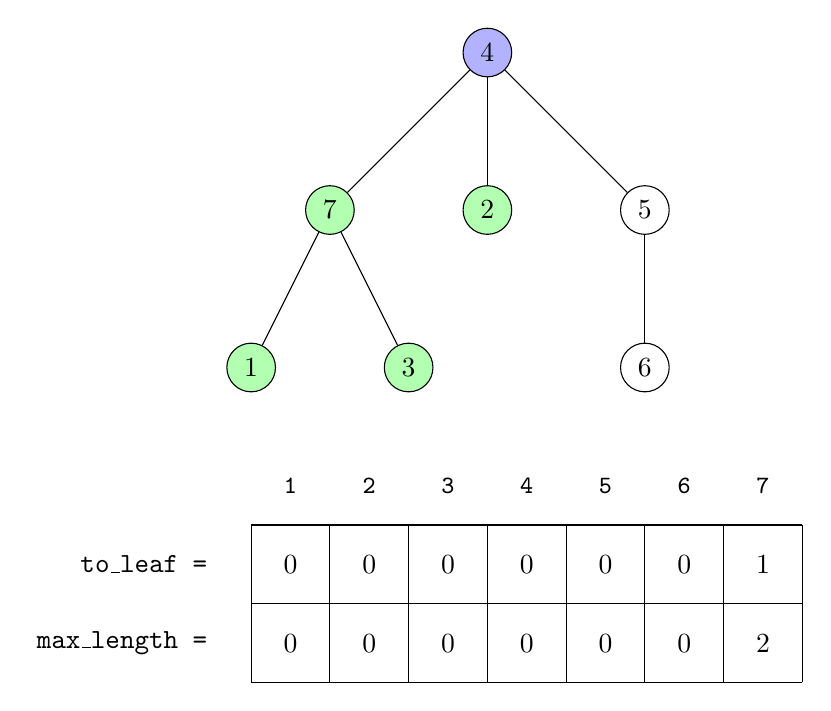
\begin{tikzpicture}

        \begin{scope}
            %\node[opacity=0] (X) at (-1, 0) { $1$ };

            \node[fill=blue!30,circle,draw] (D) at (4, 5) { $4$ };
            \node[circle,draw,fill=green!30] (C) at (2, 3) { $7$ };
            \node[circle,draw,fill=green!30] (E) at (4, 3) { $2$ };
            \node[circle,draw] (F) at (6, 3) { $5$ };
            \node[circle,draw,fill=green!30] (A) at (1, 1) { $1$ };
            \node[circle,draw,fill=green!30] (B) at (3, 1) { $3$ };
            \node[circle,draw,fill=white!30] (G) at (6, 1) { $6$ };

            \draw (A) -- (C);
            \draw (B) -- (C);
            \draw (C) -- (D);
            \draw (D) -- (E);
            \draw (D) -- (F);
            \draw (F) -- (G);

            \node[anchor=east] at (0.75, -1.5) { \texttt{to\_leaf = } };
            \draw (1, -2) grid (8, -1);

            \node[anchor=east] at (0.75, -2.5) { \texttt{max\_length = } };
            \draw (1, -3) grid (8, -2);

            \node at (1.5, -0.5) { \small \texttt{1} };
            \node at (2.5, -0.5) { \small \texttt{2} };
            \node at (3.5, -0.5) { \small \texttt{3} };
            \node at (4.5, -0.5) { \small \texttt{4} };
            \node at (5.5, -0.5) { \small \texttt{5} };
            \node at (6.5, -0.5) { \small \texttt{6} };
            \node at (7.5, -0.5) { \small \texttt{7} };

            \node at (1.5, -1.5) { \textcolor{black}{$0$} };
            \node at (2.5, -1.5) { \textcolor{black}{$0$} };
            \node at (3.5, -1.5) { \textcolor{black}{$0$} };
            \node at (4.5, -1.5) { \textcolor{black}{$0$} };
            \node at (5.5, -1.5) { $0$ };
            \node at (6.5, -1.5) { $0$ };
            \node at (7.5, -1.5) { \textcolor{black}{$1$} };

            \node at (1.5, -2.5) { \textcolor{black}{$0$} };
            \node at (2.5, -2.5) { \textcolor{black}{$0$} };
            \node at (3.5, -2.5) { \textcolor{black}{$0$} };
            \node at (4.5, -2.5) { \textcolor{black}{$0$} };
            \node at (5.5, -2.5) { $0$ };
            \node at (6.5, -2.5) { $0$ };
            \node at (7.5, -2.5) { \textcolor{black}{$2$} };


        \end{scope}
    \end{tikzpicture}

\end{frame}

\begin{frame}[fragile]{Visualização do algoritmo que computa o diâmetro com DP}

    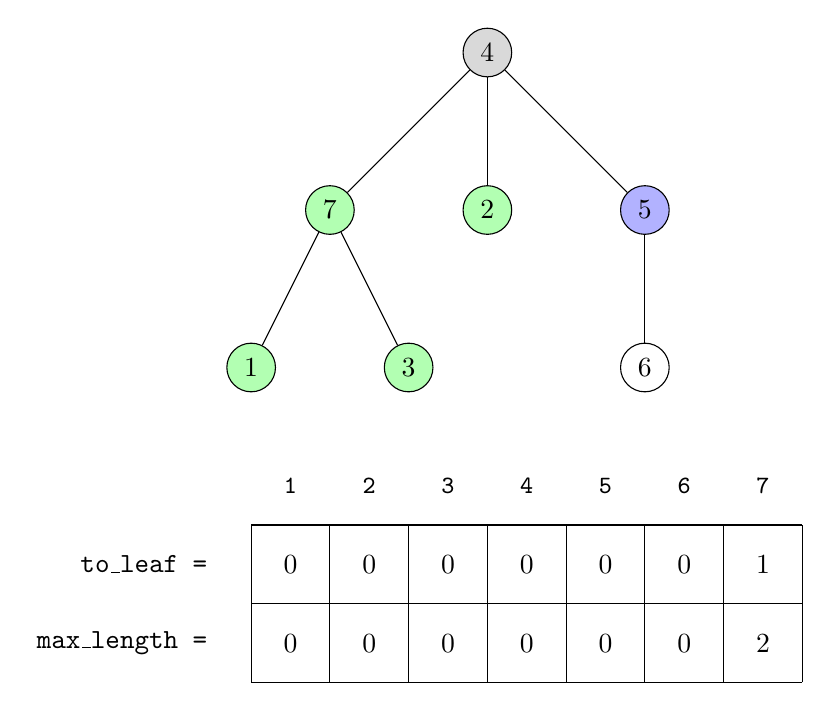
\begin{tikzpicture}

        \begin{scope}
            %\node[opacity=0] (X) at (-1, 0) { $1$ };

            \node[fill=gray!30,circle,draw] (D) at (4, 5) { $4$ };
            \node[circle,draw,fill=green!30] (C) at (2, 3) { $7$ };
            \node[circle,draw,fill=green!30] (E) at (4, 3) { $2$ };
            \node[circle,draw,fill=blue!30] (F) at (6, 3) { $5$ };
            \node[circle,draw,fill=green!30] (A) at (1, 1) { $1$ };
            \node[circle,draw,fill=green!30] (B) at (3, 1) { $3$ };
            \node[circle,draw,fill=white!30] (G) at (6, 1) { $6$ };

            \draw (A) -- (C);
            \draw (B) -- (C);
            \draw (C) -- (D);
            \draw (D) -- (E);
            \draw (D) -- (F);
            \draw (F) -- (G);

            \node[anchor=east] at (0.75, -1.5) { \texttt{to\_leaf = } };
            \draw (1, -2) grid (8, -1);

            \node[anchor=east] at (0.75, -2.5) { \texttt{max\_length = } };
            \draw (1, -3) grid (8, -2);

            \node at (1.5, -0.5) { \small \texttt{1} };
            \node at (2.5, -0.5) { \small \texttt{2} };
            \node at (3.5, -0.5) { \small \texttt{3} };
            \node at (4.5, -0.5) { \small \texttt{4} };
            \node at (5.5, -0.5) { \small \texttt{5} };
            \node at (6.5, -0.5) { \small \texttt{6} };
            \node at (7.5, -0.5) { \small \texttt{7} };

            \node at (1.5, -1.5) { \textcolor{black}{$0$} };
            \node at (2.5, -1.5) { \textcolor{black}{$0$} };
            \node at (3.5, -1.5) { \textcolor{black}{$0$} };
            \node at (4.5, -1.5) { \textcolor{black}{$0$} };
            \node at (5.5, -1.5) { $0$ };
            \node at (6.5, -1.5) { $0$ };
            \node at (7.5, -1.5) { \textcolor{black}{$1$} };

            \node at (1.5, -2.5) { \textcolor{black}{$0$} };
            \node at (2.5, -2.5) { \textcolor{black}{$0$} };
            \node at (3.5, -2.5) { \textcolor{black}{$0$} };
            \node at (4.5, -2.5) { \textcolor{black}{$0$} };
            \node at (5.5, -2.5) { $0$ };
            \node at (6.5, -2.5) { $0$ };
            \node at (7.5, -2.5) { \textcolor{black}{$2$} };


        \end{scope}
    \end{tikzpicture}

\end{frame}

\begin{frame}[fragile]{Visualização do algoritmo que computa o diâmetro com DP}

    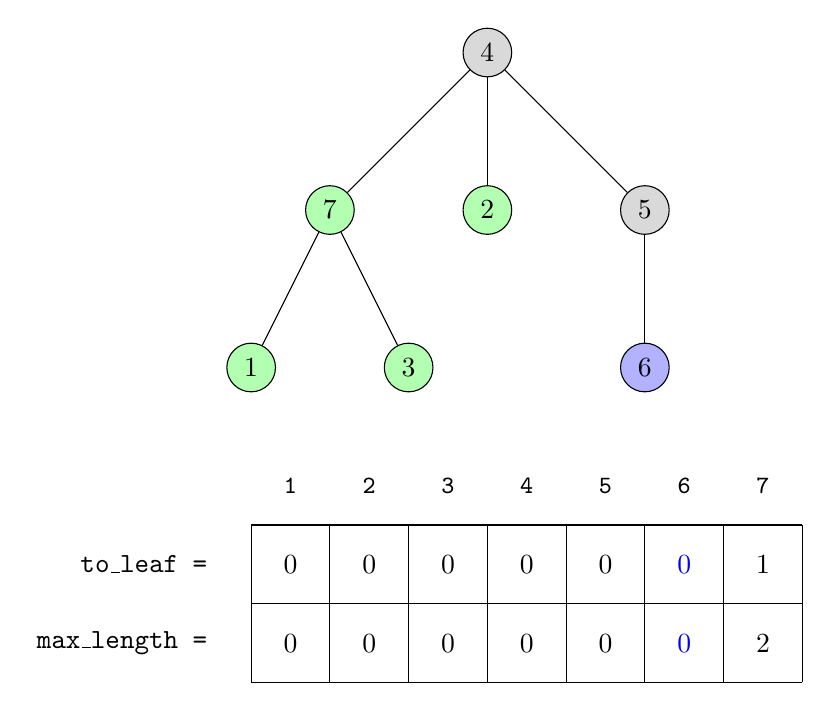
\begin{tikzpicture}

        \begin{scope}
            %\node[opacity=0] (X) at (-1, 0) { $1$ };

            \node[fill=gray!30,circle,draw] (D) at (4, 5) { $4$ };
            \node[circle,draw,fill=green!30] (C) at (2, 3) { $7$ };
            \node[circle,draw,fill=green!30] (E) at (4, 3) { $2$ };
            \node[circle,draw,fill=gray!30] (F) at (6, 3) { $5$ };
            \node[circle,draw,fill=green!30] (A) at (1, 1) { $1$ };
            \node[circle,draw,fill=green!30] (B) at (3, 1) { $3$ };
            \node[circle,draw,fill=blue!30] (G) at (6, 1) { $6$ };

            \draw (A) -- (C);
            \draw (B) -- (C);
            \draw (C) -- (D);
            \draw (D) -- (E);
            \draw (D) -- (F);
            \draw (F) -- (G);

            \node[anchor=east] at (0.75, -1.5) { \texttt{to\_leaf = } };
            \draw (1, -2) grid (8, -1);

            \node[anchor=east] at (0.75, -2.5) { \texttt{max\_length = } };
            \draw (1, -3) grid (8, -2);

            \node at (1.5, -0.5) { \small \texttt{1} };
            \node at (2.5, -0.5) { \small \texttt{2} };
            \node at (3.5, -0.5) { \small \texttt{3} };
            \node at (4.5, -0.5) { \small \texttt{4} };
            \node at (5.5, -0.5) { \small \texttt{5} };
            \node at (6.5, -0.5) { \small \texttt{6} };
            \node at (7.5, -0.5) { \small \texttt{7} };

            \node at (1.5, -1.5) { \textcolor{black}{$0$} };
            \node at (2.5, -1.5) { \textcolor{black}{$0$} };
            \node at (3.5, -1.5) { \textcolor{black}{$0$} };
            \node at (4.5, -1.5) { \textcolor{black}{$0$} };
            \node at (5.5, -1.5) { $0$ };
            \node at (6.5, -1.5) { \textcolor{blue}{$0$} };
            \node at (7.5, -1.5) { \textcolor{black}{$1$} };

            \node at (1.5, -2.5) { \textcolor{black}{$0$} };
            \node at (2.5, -2.5) { \textcolor{black}{$0$} };
            \node at (3.5, -2.5) { \textcolor{black}{$0$} };
            \node at (4.5, -2.5) { \textcolor{black}{$0$} };
            \node at (5.5, -2.5) { $0$ };
            \node at (6.5, -2.5) { \textcolor{blue}{$0$} };
            \node at (7.5, -2.5) { \textcolor{black}{$2$} };


        \end{scope}
    \end{tikzpicture}

\end{frame}

\begin{frame}[fragile]{Visualização do algoritmo que computa o diâmetro com DP}

    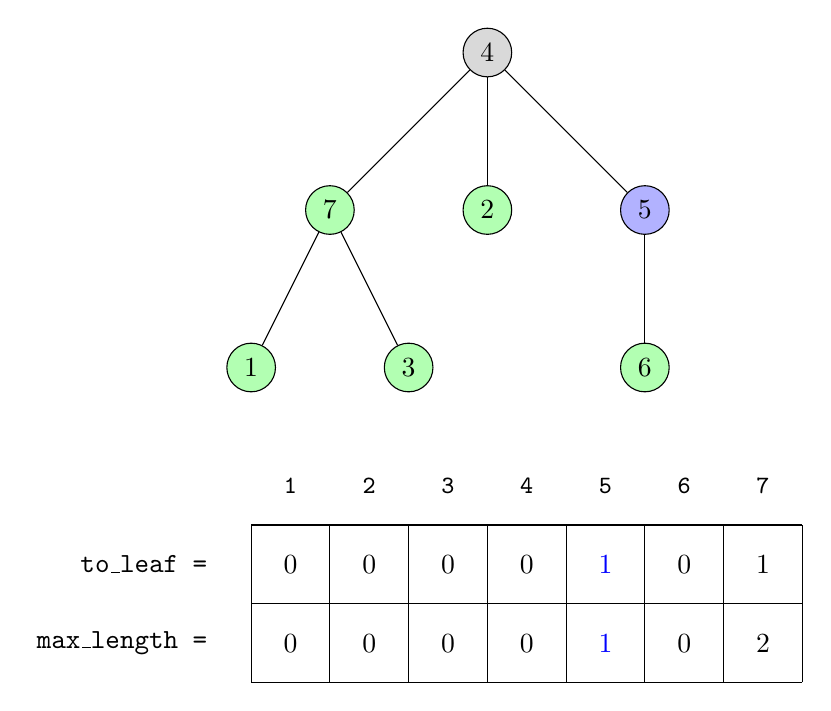
\begin{tikzpicture}

        \begin{scope}
            %\node[opacity=0] (X) at (-1, 0) { $1$ };

            \node[fill=gray!30,circle,draw] (D) at (4, 5) { $4$ };
            \node[circle,draw,fill=green!30] (C) at (2, 3) { $7$ };
            \node[circle,draw,fill=green!30] (E) at (4, 3) { $2$ };
            \node[circle,draw,fill=blue!30] (F) at (6, 3) { $5$ };
            \node[circle,draw,fill=green!30] (A) at (1, 1) { $1$ };
            \node[circle,draw,fill=green!30] (B) at (3, 1) { $3$ };
            \node[circle,draw,fill=green!30] (G) at (6, 1) { $6$ };

            \draw (A) -- (C);
            \draw (B) -- (C);
            \draw (C) -- (D);
            \draw (D) -- (E);
            \draw (D) -- (F);
            \draw (F) -- (G);

            \node[anchor=east] at (0.75, -1.5) { \texttt{to\_leaf = } };
            \draw (1, -2) grid (8, -1);

            \node[anchor=east] at (0.75, -2.5) { \texttt{max\_length = } };
            \draw (1, -3) grid (8, -2);

            \node at (1.5, -0.5) { \small \texttt{1} };
            \node at (2.5, -0.5) { \small \texttt{2} };
            \node at (3.5, -0.5) { \small \texttt{3} };
            \node at (4.5, -0.5) { \small \texttt{4} };
            \node at (5.5, -0.5) { \small \texttt{5} };
            \node at (6.5, -0.5) { \small \texttt{6} };
            \node at (7.5, -0.5) { \small \texttt{7} };

            \node at (1.5, -1.5) { \textcolor{black}{$0$} };
            \node at (2.5, -1.5) { \textcolor{black}{$0$} };
            \node at (3.5, -1.5) { \textcolor{black}{$0$} };
            \node at (4.5, -1.5) { \textcolor{black}{$0$} };
            \node at (5.5, -1.5) { \textcolor{blue}{$1$} };
            \node at (6.5, -1.5) { \textcolor{black}{$0$} };
            \node at (7.5, -1.5) { \textcolor{black}{$1$} };

            \node at (1.5, -2.5) { \textcolor{black}{$0$} };
            \node at (2.5, -2.5) { \textcolor{black}{$0$} };
            \node at (3.5, -2.5) { \textcolor{black}{$0$} };
            \node at (4.5, -2.5) { \textcolor{black}{$0$} };
            \node at (5.5, -2.5) { \textcolor{blue}{$1$} };
            \node at (6.5, -2.5) { \textcolor{black}{$0$} };
            \node at (7.5, -2.5) { \textcolor{black}{$2$} };


        \end{scope}
    \end{tikzpicture}

\end{frame}

\begin{frame}[fragile]{Visualização do algoritmo que computa o diâmetro com DP}

    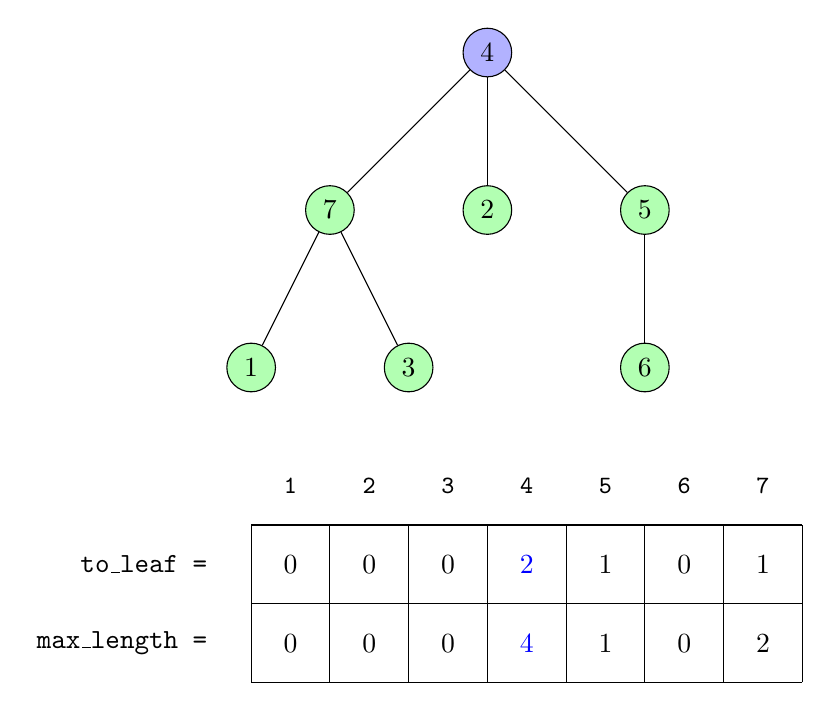
\begin{tikzpicture}

        \begin{scope}
            %\node[opacity=0] (X) at (-1, 0) { $1$ };

            \node[fill=blue!30,circle,draw] (D) at (4, 5) { $4$ };
            \node[circle,draw,fill=green!30] (C) at (2, 3) { $7$ };
            \node[circle,draw,fill=green!30] (E) at (4, 3) { $2$ };
            \node[circle,draw,fill=green!30] (F) at (6, 3) { $5$ };
            \node[circle,draw,fill=green!30] (A) at (1, 1) { $1$ };
            \node[circle,draw,fill=green!30] (B) at (3, 1) { $3$ };
            \node[circle,draw,fill=green!30] (G) at (6, 1) { $6$ };

            \draw (A) -- (C);
            \draw (B) -- (C);
            \draw (C) -- (D);
            \draw (D) -- (E);
            \draw (D) -- (F);
            \draw (F) -- (G);

            \node[anchor=east] at (0.75, -1.5) { \texttt{to\_leaf = } };
            \draw (1, -2) grid (8, -1);

            \node[anchor=east] at (0.75, -2.5) { \texttt{max\_length = } };
            \draw (1, -3) grid (8, -2);

            \node at (1.5, -0.5) { \small \texttt{1} };
            \node at (2.5, -0.5) { \small \texttt{2} };
            \node at (3.5, -0.5) { \small \texttt{3} };
            \node at (4.5, -0.5) { \small \texttt{4} };
            \node at (5.5, -0.5) { \small \texttt{5} };
            \node at (6.5, -0.5) { \small \texttt{6} };
            \node at (7.5, -0.5) { \small \texttt{7} };

            \node at (1.5, -1.5) { \textcolor{black}{$0$} };
            \node at (2.5, -1.5) { \textcolor{black}{$0$} };
            \node at (3.5, -1.5) { \textcolor{black}{$0$} };
            \node at (4.5, -1.5) { \textcolor{blue}{$2$} };
            \node at (5.5, -1.5) { \textcolor{black}{$1$} };
            \node at (6.5, -1.5) { \textcolor{black}{$0$} };
            \node at (7.5, -1.5) { \textcolor{black}{$1$} };

            \node at (1.5, -2.5) { \textcolor{black}{$0$} };
            \node at (2.5, -2.5) { \textcolor{black}{$0$} };
            \node at (3.5, -2.5) { \textcolor{black}{$0$} };
            \node at (4.5, -2.5) { \textcolor{blue}{$4$} };
            \node at (5.5, -2.5) { \textcolor{black}{$1$} };
            \node at (6.5, -2.5) { \textcolor{black}{$0$} };
            \node at (7.5, -2.5) { \textcolor{black}{$2$} };


        \end{scope}
    \end{tikzpicture}

\end{frame}

\begin{frame}[fragile]{Visualização do algoritmo que computa o diâmetro com DP}

    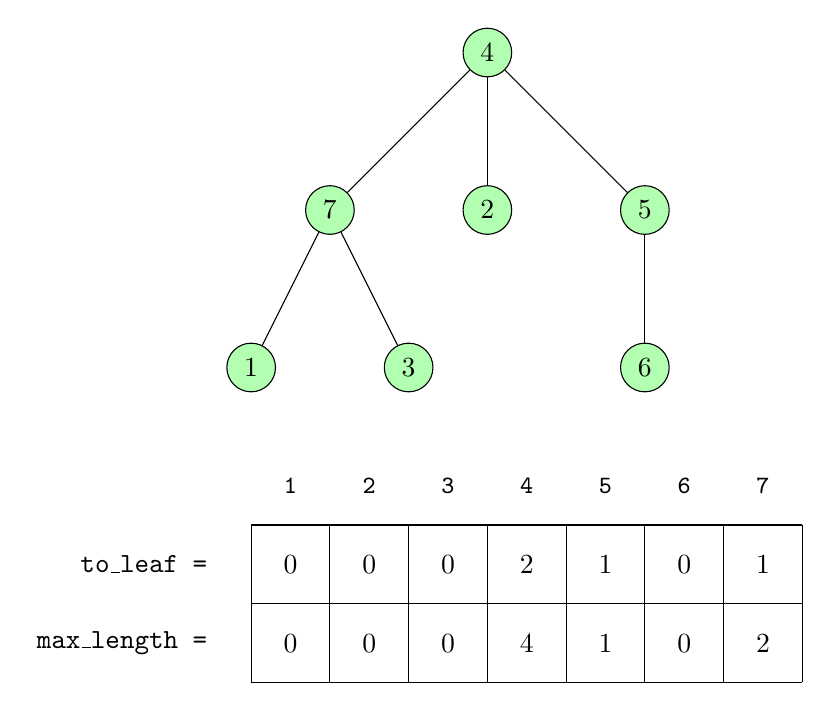
\begin{tikzpicture}

        \begin{scope}
            %\node[opacity=0] (X) at (-1, 0) { $1$ };

            \node[fill=green!30,circle,draw] (D) at (4, 5) { $4$ };
            \node[circle,draw,fill=green!30] (C) at (2, 3) { $7$ };
            \node[circle,draw,fill=green!30] (E) at (4, 3) { $2$ };
            \node[circle,draw,fill=green!30] (F) at (6, 3) { $5$ };
            \node[circle,draw,fill=green!30] (A) at (1, 1) { $1$ };
            \node[circle,draw,fill=green!30] (B) at (3, 1) { $3$ };
            \node[circle,draw,fill=green!30] (G) at (6, 1) { $6$ };

            \draw (A) -- (C);
            \draw (B) -- (C);
            \draw (C) -- (D);
            \draw (D) -- (E);
            \draw (D) -- (F);
            \draw (F) -- (G);

            \node[anchor=east] at (0.75, -1.5) { \texttt{to\_leaf = } };
            \draw (1, -2) grid (8, -1);

            \node[anchor=east] at (0.75, -2.5) { \texttt{max\_length = } };
            \draw (1, -3) grid (8, -2);

            \node at (1.5, -0.5) { \small \texttt{1} };
            \node at (2.5, -0.5) { \small \texttt{2} };
            \node at (3.5, -0.5) { \small \texttt{3} };
            \node at (4.5, -0.5) { \small \texttt{4} };
            \node at (5.5, -0.5) { \small \texttt{5} };
            \node at (6.5, -0.5) { \small \texttt{6} };
            \node at (7.5, -0.5) { \small \texttt{7} };

            \node at (1.5, -1.5) { \textcolor{black}{$0$} };
            \node at (2.5, -1.5) { \textcolor{black}{$0$} };
            \node at (3.5, -1.5) { \textcolor{black}{$0$} };
            \node at (4.5, -1.5) { \textcolor{black}{$2$} };
            \node at (5.5, -1.5) { \textcolor{black}{$1$} };
            \node at (6.5, -1.5) { \textcolor{black}{$0$} };
            \node at (7.5, -1.5) { \textcolor{black}{$1$} };

            \node at (1.5, -2.5) { \textcolor{black}{$0$} };
            \node at (2.5, -2.5) { \textcolor{black}{$0$} };
            \node at (3.5, -2.5) { \textcolor{black}{$0$} };
            \node at (4.5, -2.5) { \textcolor{black}{$4$} };
            \node at (5.5, -2.5) { \textcolor{black}{$1$} };
            \node at (6.5, -2.5) { \textcolor{black}{$0$} };
            \node at (7.5, -2.5) { \textcolor{black}{$2$} };


        \end{scope}
    \end{tikzpicture}

\end{frame}

\begin{frame}[fragile]{Implementação da rotina que computa o diâmetro com DP}
    \inputsnippet{c++}{1}{21}{dp.cpp}
\end{frame}

\begin{frame}[fragile]{Implementação da rotina que computa o diâmetro com DP}
    \inputsnippet{c++}{22}{40}{dp.cpp}
\end{frame}

\begin{frame}[fragile]{Implementação da rotina que computa o diâmetro com DP}
    \inputsnippet{c++}{41}{61}{dp.cpp}
\end{frame}

\begin{frame}[fragile]{Implementação da rotina que computa o diâmetro com DP}
    \inputsnippet{c++}{62}{82}{dp.cpp}
\end{frame}

\begin{frame}[fragile]{Diâmetro com DFS}

    \begin{itemize}
        \item Computar o diâmetro usando DFS é simples de implementar, mas a corretude do
            algoritmo não é trivial

        \item Basta escolher dois vértices distintos $u$ e $v$ quaisquer

        \item Em seguida, identifique o vértice $w$ mais distante de $u$

        \item Agora, compute o vértice $t$ mais distante de $w$

        \item O diâmetro será a distância entre $w$ e $t$

        \item A corretude é provada em duas etapas

        \item Primeiro, mostre que ao menos um vértice $x$ do caminho de $u$ a $w$ deve
            fazer parte de um caminho cujo tamanho é o diâmetro

        \item Em seguida, use este fato para provar que $w$ deve ser o extremo de um caminho 
            máximo

        \item Ambos fatos podem ser demonstrados por contradição
    \end{itemize}

\end{frame}

\begin{frame}[fragile]{Visualização do algoritmo que computa o diâmetro com DFS}

    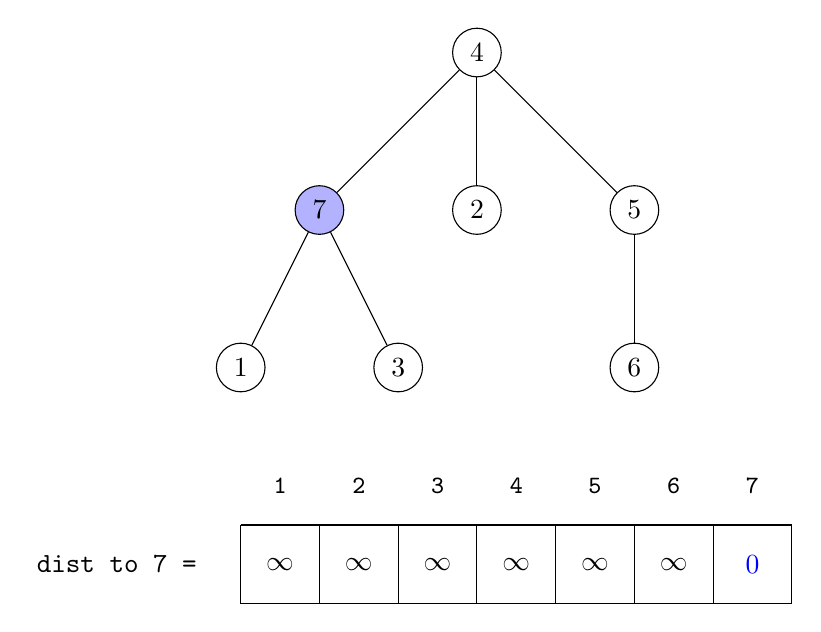
\begin{tikzpicture}

        \begin{scope}
            %\node[opacity=0] (X) at (-1, 0) { $1$ };

            \node[fill=white!30,circle,draw] (D) at (4, 5) { $4$ };
            \node[circle,draw,fill=blue!30] (C) at (2, 3) { $7$ };
            \node[circle,draw,fill=white!30] (E) at (4, 3) { $2$ };
            \node[circle,draw] (F) at (6, 3) { $5$ };
            \node[circle,draw,fill=white!30] (A) at (1, 1) { $1$ };
            \node[circle,draw,fill=white!30] (B) at (3, 1) { $3$ };
            \node[circle,draw,fill=white!30] (G) at (6, 1) { $6$ };

            \draw (A) -- (C);
            \draw (B) -- (C);
            \draw (C) -- (D);
            \draw (D) -- (E);
            \draw (D) -- (F);
            \draw (F) -- (G);

            \node[anchor=east] at (0.75, -1.5) { \texttt{dist to 7 = } };
            \draw (1, -2) grid (8, -1);

            \node at (1.5, -0.5) { \small \texttt{1} };
            \node at (2.5, -0.5) { \small \texttt{2} };
            \node at (3.5, -0.5) { \small \texttt{3} };
            \node at (4.5, -0.5) { \small \texttt{4} };
            \node at (5.5, -0.5) { \small \texttt{5} };
            \node at (6.5, -0.5) { \small \texttt{6} };
            \node at (7.5, -0.5) { \small \texttt{7} };

            \node at (1.5, -1.5) { $\infty$ };
            \node at (2.5, -1.5) { $\infty$ };
            \node at (3.5, -1.5) { $\infty$ };
            \node at (4.5, -1.5) { \textcolor{black}{$\infty$} };
            \node at (5.5, -1.5) { $\infty$ };
            \node at (6.5, -1.5) { $\infty$ };
            \node at (7.5, -1.5) { \textcolor{blue}{$0$} };
        \end{scope}
    \end{tikzpicture}

\end{frame}


\begin{frame}[fragile]{Visualização do algoritmo que computa o diâmetro com DFS}

    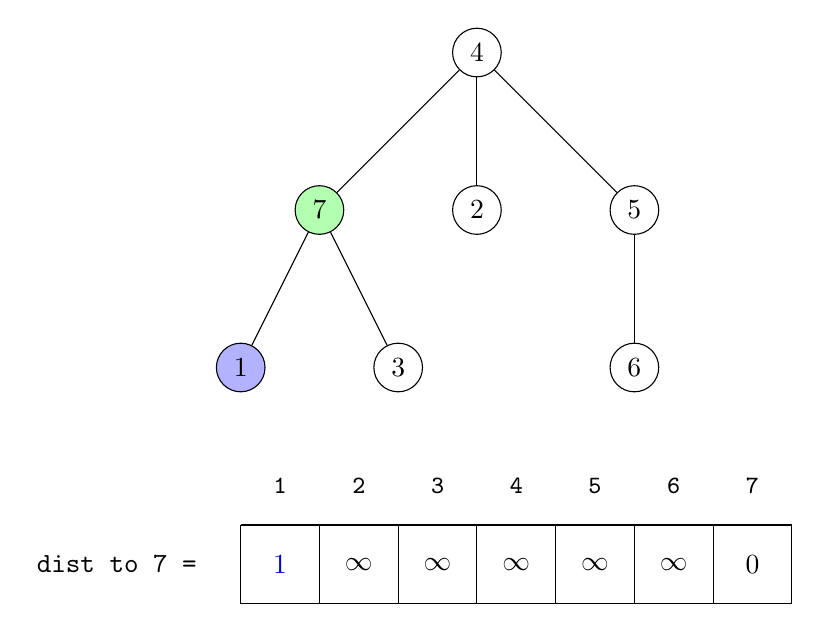
\begin{tikzpicture}

        \begin{scope}
            %\node[opacity=0] (X) at (-1, 0) { $1$ };

            \node[fill=white!30,circle,draw] (D) at (4, 5) { $4$ };
            \node[circle,draw,fill=green!30] (C) at (2, 3) { $7$ };
            \node[circle,draw,fill=white!30] (E) at (4, 3) { $2$ };
            \node[circle,draw] (F) at (6, 3) { $5$ };
            \node[circle,draw,fill=blue!30] (A) at (1, 1) { $1$ };
            \node[circle,draw,fill=white!30] (B) at (3, 1) { $3$ };
            \node[circle,draw,fill=white!30] (G) at (6, 1) { $6$ };

            \draw (A) -- (C);
            \draw (B) -- (C);
            \draw (C) -- (D);
            \draw (D) -- (E);
            \draw (D) -- (F);
            \draw (F) -- (G);

            \node[anchor=east] at (0.75, -1.5) { \texttt{dist to 7 = } };
            \draw (1, -2) grid (8, -1);

            \node at (1.5, -0.5) { \small \texttt{1} };
            \node at (2.5, -0.5) { \small \texttt{2} };
            \node at (3.5, -0.5) { \small \texttt{3} };
            \node at (4.5, -0.5) { \small \texttt{4} };
            \node at (5.5, -0.5) { \small \texttt{5} };
            \node at (6.5, -0.5) { \small \texttt{6} };
            \node at (7.5, -0.5) { \small \texttt{7} };

            \node at (1.5, -1.5) { \textcolor{blue}{$1$} };
            \node at (2.5, -1.5) { $\infty$ };
            \node at (3.5, -1.5) { \textcolor{black}{$\infty$} };
            \node at (4.5, -1.5) { \textcolor{black}{$\infty$} };
            \node at (5.5, -1.5) { $\infty$ };
            \node at (6.5, -1.5) { $\infty$ };
            \node at (7.5, -1.5) { \textcolor{black}{$0$} };
        \end{scope}
    \end{tikzpicture}

\end{frame}

\begin{frame}[fragile]{Visualização do algoritmo que computa o diâmetro com DFS}

    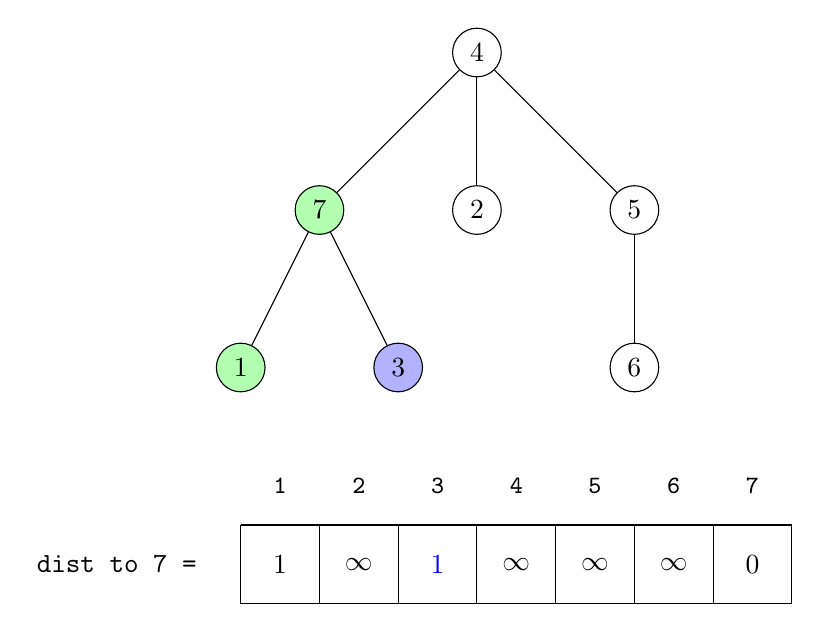
\begin{tikzpicture}

        \begin{scope}
            %\node[opacity=0] (X) at (-1, 0) { $1$ };

            \node[fill=white!30,circle,draw] (D) at (4, 5) { $4$ };
            \node[circle,draw,fill=green!30] (C) at (2, 3) { $7$ };
            \node[circle,draw,fill=white!30] (E) at (4, 3) { $2$ };
            \node[circle,draw] (F) at (6, 3) { $5$ };
            \node[circle,draw,fill=green!30] (A) at (1, 1) { $1$ };
            \node[circle,draw,fill=blue!30] (B) at (3, 1) { $3$ };
            \node[circle,draw,fill=white!30] (G) at (6, 1) { $6$ };

            \draw (A) -- (C);
            \draw (B) -- (C);
            \draw (C) -- (D);
            \draw (D) -- (E);
            \draw (D) -- (F);
            \draw (F) -- (G);

            \node[anchor=east] at (0.75, -1.5) { \texttt{dist to 7 = } };
            \draw (1, -2) grid (8, -1);

            \node at (1.5, -0.5) { \small \texttt{1} };
            \node at (2.5, -0.5) { \small \texttt{2} };
            \node at (3.5, -0.5) { \small \texttt{3} };
            \node at (4.5, -0.5) { \small \texttt{4} };
            \node at (5.5, -0.5) { \small \texttt{5} };
            \node at (6.5, -0.5) { \small \texttt{6} };
            \node at (7.5, -0.5) { \small \texttt{7} };

            \node at (1.5, -1.5) { $1$ };
            \node at (2.5, -1.5) { $\infty$ };
            \node at (3.5, -1.5) { \textcolor{blue}{$1$} };
            \node at (4.5, -1.5) { \textcolor{black}{$\infty$} };
            \node at (5.5, -1.5) { $\infty$ };
            \node at (6.5, -1.5) { $\infty$ };
            \node at (7.5, -1.5) { \textcolor{black}{$0$} };
        \end{scope}
    \end{tikzpicture}

\end{frame}

\begin{frame}[fragile]{Visualização do algoritmo que computa o diâmetro com DFS}

    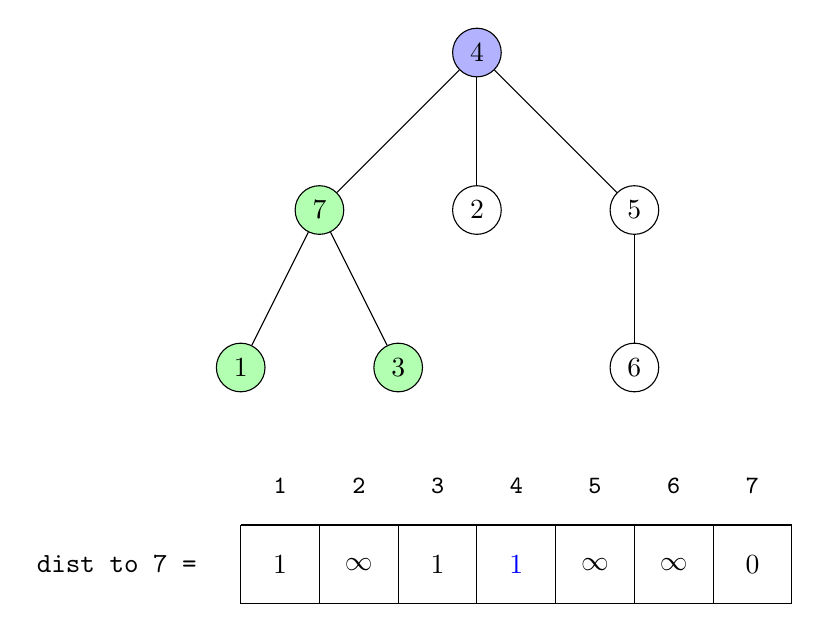
\begin{tikzpicture}

        \begin{scope}
            %\node[opacity=0] (X) at (-1, 0) { $1$ };

            \node[fill=blue!30,circle,draw] (D) at (4, 5) { $4$ };
            \node[circle,draw,fill=green!30] (C) at (2, 3) { $7$ };
            \node[circle,draw,fill=white!30] (E) at (4, 3) { $2$ };
            \node[circle,draw] (F) at (6, 3) { $5$ };
            \node[circle,draw,fill=green!30] (A) at (1, 1) { $1$ };
            \node[circle,draw,fill=green!30] (B) at (3, 1) { $3$ };
            \node[circle,draw,fill=white!30] (G) at (6, 1) { $6$ };

            \draw (A) -- (C);
            \draw (B) -- (C);
            \draw (C) -- (D);
            \draw (D) -- (E);
            \draw (D) -- (F);
            \draw (F) -- (G);

            \node[anchor=east] at (0.75, -1.5) { \texttt{dist to 7 = } };
            \draw (1, -2) grid (8, -1);

            \node at (1.5, -0.5) { \small \texttt{1} };
            \node at (2.5, -0.5) { \small \texttt{2} };
            \node at (3.5, -0.5) { \small \texttt{3} };
            \node at (4.5, -0.5) { \small \texttt{4} };
            \node at (5.5, -0.5) { \small \texttt{5} };
            \node at (6.5, -0.5) { \small \texttt{6} };
            \node at (7.5, -0.5) { \small \texttt{7} };

            \node at (1.5, -1.5) { $1$ };
            \node at (2.5, -1.5) { $\infty$ };
            \node at (3.5, -1.5) { \textcolor{black}{$1$} };
            \node at (4.5, -1.5) { \textcolor{blue}{$1$} };
            \node at (5.5, -1.5) { $\infty$ };
            \node at (6.5, -1.5) { $\infty$ };
            \node at (7.5, -1.5) { \textcolor{black}{$0$} };
        \end{scope}
    \end{tikzpicture}

\end{frame}

\begin{frame}[fragile]{Visualização do algoritmo que computa o diâmetro com DFS}

    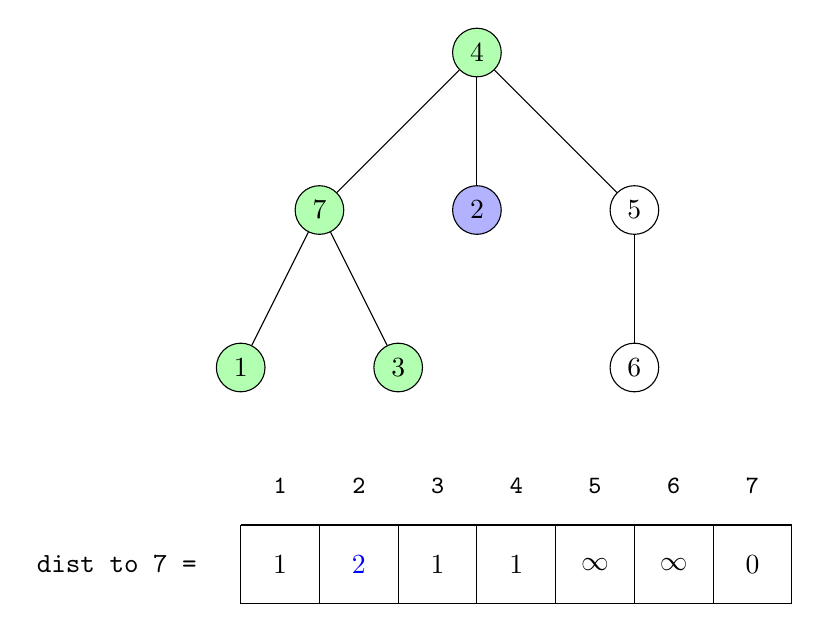
\begin{tikzpicture}

        \begin{scope}
            %\node[opacity=0] (X) at (-1, 0) { $1$ };

            \node[fill=green!30,circle,draw] (D) at (4, 5) { $4$ };
            \node[circle,draw,fill=green!30] (C) at (2, 3) { $7$ };
            \node[circle,draw,fill=blue!30] (E) at (4, 3) { $2$ };
            \node[circle,draw] (F) at (6, 3) { $5$ };
            \node[circle,draw,fill=green!30] (A) at (1, 1) { $1$ };
            \node[circle,draw,fill=green!30] (B) at (3, 1) { $3$ };
            \node[circle,draw,fill=white!30] (G) at (6, 1) { $6$ };

            \draw (A) -- (C);
            \draw (B) -- (C);
            \draw (C) -- (D);
            \draw (D) -- (E);
            \draw (D) -- (F);
            \draw (F) -- (G);

            \node[anchor=east] at (0.75, -1.5) { \texttt{dist to 7 = } };
            \draw (1, -2) grid (8, -1);

            \node at (1.5, -0.5) { \small \texttt{1} };
            \node at (2.5, -0.5) { \small \texttt{2} };
            \node at (3.5, -0.5) { \small \texttt{3} };
            \node at (4.5, -0.5) { \small \texttt{4} };
            \node at (5.5, -0.5) { \small \texttt{5} };
            \node at (6.5, -0.5) { \small \texttt{6} };
            \node at (7.5, -0.5) { \small \texttt{7} };

            \node at (1.5, -1.5) { $1$ };
            \node at (2.5, -1.5) { \textcolor{blue}{$2$} };
            \node at (3.5, -1.5) { \textcolor{black}{$1$} };
            \node at (4.5, -1.5) { \textcolor{black}{$1$} };
            \node at (5.5, -1.5) { $\infty$ };
            \node at (6.5, -1.5) { $\infty$ };
            \node at (7.5, -1.5) { \textcolor{black}{$0$} };
        \end{scope}
    \end{tikzpicture}

\end{frame}

\begin{frame}[fragile]{Visualização do algoritmo que computa o diâmetro com DFS}

    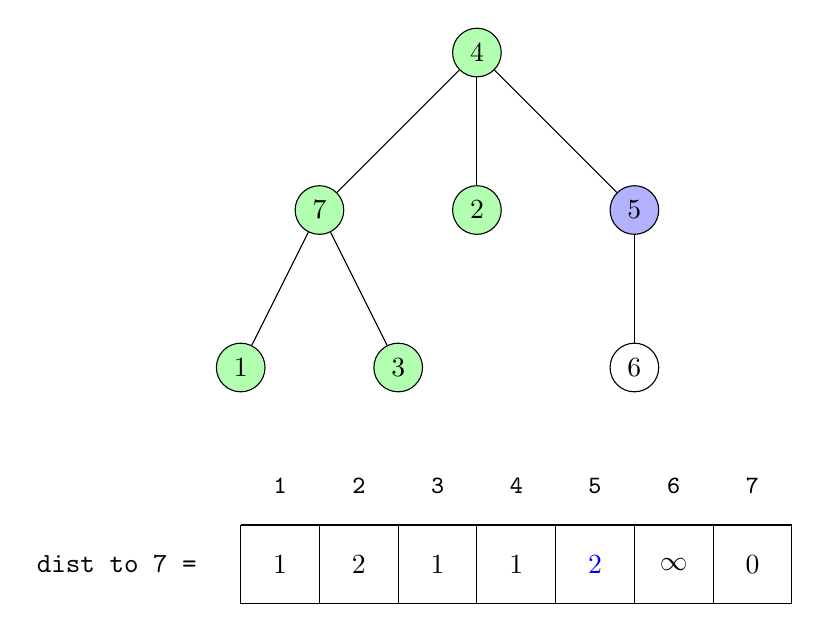
\begin{tikzpicture}

        \begin{scope}
            %\node[opacity=0] (X) at (-1, 0) { $1$ };

            \node[fill=green!30,circle,draw] (D) at (4, 5) { $4$ };
            \node[circle,draw,fill=green!30] (C) at (2, 3) { $7$ };
            \node[circle,draw,fill=green!30] (E) at (4, 3) { $2$ };
            \node[circle,draw,fill=blue!30] (F) at (6, 3) { $5$ };
            \node[circle,draw,fill=green!30] (A) at (1, 1) { $1$ };
            \node[circle,draw,fill=green!30] (B) at (3, 1) { $3$ };
            \node[circle,draw,fill=white!30] (G) at (6, 1) { $6$ };

            \draw (A) -- (C);
            \draw (B) -- (C);
            \draw (C) -- (D);
            \draw (D) -- (E);
            \draw (D) -- (F);
            \draw (F) -- (G);

            \node[anchor=east] at (0.75, -1.5) { \texttt{dist to 7 = } };
            \draw (1, -2) grid (8, -1);

            \node at (1.5, -0.5) { \small \texttt{1} };
            \node at (2.5, -0.5) { \small \texttt{2} };
            \node at (3.5, -0.5) { \small \texttt{3} };
            \node at (4.5, -0.5) { \small \texttt{4} };
            \node at (5.5, -0.5) { \small \texttt{5} };
            \node at (6.5, -0.5) { \small \texttt{6} };
            \node at (7.5, -0.5) { \small \texttt{7} };

            \node at (1.5, -1.5) { $1$ };
            \node at (2.5, -1.5) { \textcolor{black}{$2$} };
            \node at (3.5, -1.5) { \textcolor{black}{$1$} };
            \node at (4.5, -1.5) { \textcolor{black}{$1$} };
            \node at (5.5, -1.5) { \textcolor{blue}{$2$} };
            \node at (6.5, -1.5) { $\infty$ };
            \node at (7.5, -1.5) { \textcolor{black}{$0$} };
        \end{scope}
    \end{tikzpicture}

\end{frame}

\begin{frame}[fragile]{Visualização do algoritmo que computa o diâmetro com DFS}

    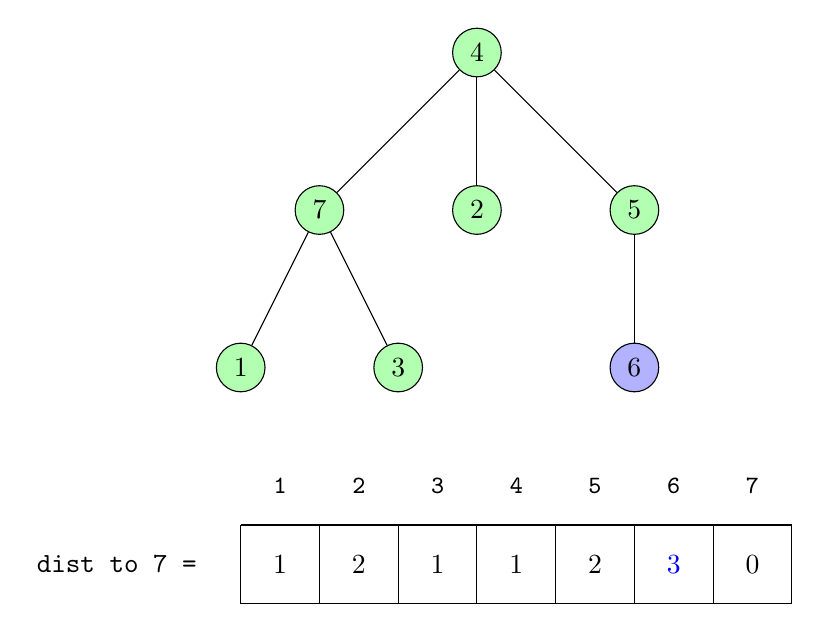
\begin{tikzpicture}

        \begin{scope}
            %\node[opacity=0] (X) at (-1, 0) { $1$ };

            \node[fill=green!30,circle,draw] (D) at (4, 5) { $4$ };
            \node[circle,draw,fill=green!30] (C) at (2, 3) { $7$ };
            \node[circle,draw,fill=green!30] (E) at (4, 3) { $2$ };
            \node[circle,draw,fill=green!30] (F) at (6, 3) { $5$ };
            \node[circle,draw,fill=green!30] (A) at (1, 1) { $1$ };
            \node[circle,draw,fill=green!30] (B) at (3, 1) { $3$ };
            \node[circle,draw,fill=blue!30] (G) at (6, 1) { $6$ };

            \draw (A) -- (C);
            \draw (B) -- (C);
            \draw (C) -- (D);
            \draw (D) -- (E);
            \draw (D) -- (F);
            \draw (F) -- (G);

            \node[anchor=east] at (0.75, -1.5) { \texttt{dist to 7 = } };
            \draw (1, -2) grid (8, -1);

            \node at (1.5, -0.5) { \small \texttt{1} };
            \node at (2.5, -0.5) { \small \texttt{2} };
            \node at (3.5, -0.5) { \small \texttt{3} };
            \node at (4.5, -0.5) { \small \texttt{4} };
            \node at (5.5, -0.5) { \small \texttt{5} };
            \node at (6.5, -0.5) { \small \texttt{6} };
            \node at (7.5, -0.5) { \small \texttt{7} };

            \node at (1.5, -1.5) { $1$ };
            \node at (2.5, -1.5) { \textcolor{black}{$2$} };
            \node at (3.5, -1.5) { \textcolor{black}{$1$} };
            \node at (4.5, -1.5) { \textcolor{black}{$1$} };
            \node at (5.5, -1.5) { \textcolor{black}{$2$} };
            \node at (6.5, -1.5) { \textcolor{blue}{$3$} };
            \node at (7.5, -1.5) { \textcolor{black}{$0$} };
        \end{scope}
    \end{tikzpicture}

\end{frame}

\begin{frame}[fragile]{Visualização do algoritmo que computa o diâmetro com DFS}

    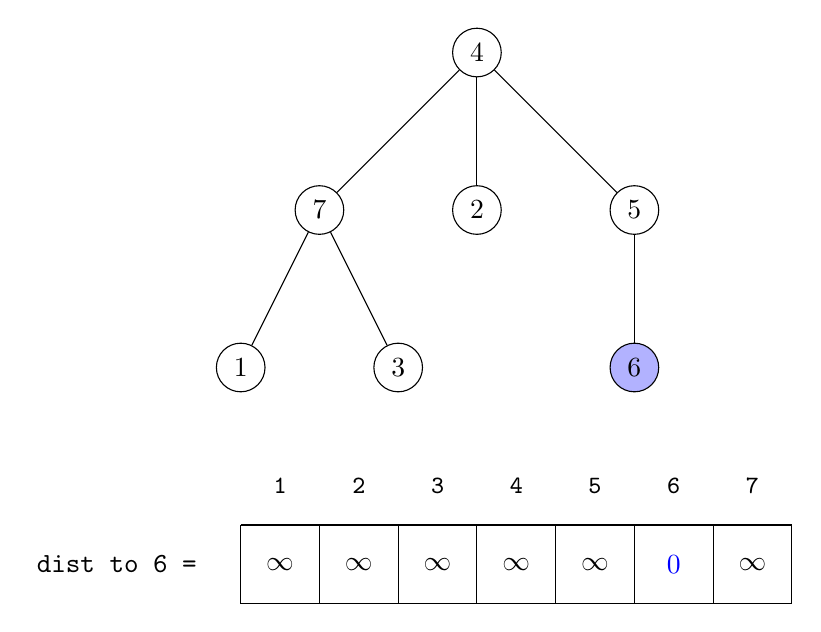
\begin{tikzpicture}

        \begin{scope}
            %\node[opacity=0] (X) at (-1, 0) { $1$ };

            \node[fill=white!30,circle,draw] (D) at (4, 5) { $4$ };
            \node[circle,draw,fill=white!30] (C) at (2, 3) { $7$ };
            \node[circle,draw,fill=white!30] (E) at (4, 3) { $2$ };
            \node[circle,draw,fill=white!30] (F) at (6, 3) { $5$ };
            \node[circle,draw,fill=white!30] (A) at (1, 1) { $1$ };
            \node[circle,draw,fill=white!30] (B) at (3, 1) { $3$ };
            \node[circle,draw,fill=blue!30] (G) at (6, 1) { $6$ };

            \draw (A) -- (C);
            \draw (B) -- (C);
            \draw (C) -- (D);
            \draw (D) -- (E);
            \draw (D) -- (F);
            \draw (F) -- (G);

            \node[anchor=east] at (0.75, -1.5) { \texttt{dist to 6 = } };
            \draw (1, -2) grid (8, -1);

            \node at (1.5, -0.5) { \small \texttt{1} };
            \node at (2.5, -0.5) { \small \texttt{2} };
            \node at (3.5, -0.5) { \small \texttt{3} };
            \node at (4.5, -0.5) { \small \texttt{4} };
            \node at (5.5, -0.5) { \small \texttt{5} };
            \node at (6.5, -0.5) { \small \texttt{6} };
            \node at (7.5, -0.5) { \small \texttt{7} };

            \node at (1.5, -1.5) { \textcolor{black}{$\infty$} };
            \node at (2.5, -1.5) { \textcolor{black}{$\infty$} };
            \node at (3.5, -1.5) { \textcolor{black}{$\infty$} };
            \node at (4.5, -1.5) { \textcolor{black}{$\infty$} };
            \node at (5.5, -1.5) { \textcolor{black}{$\infty$} };
            \node at (6.5, -1.5) { \textcolor{blue}{$0$} };
            \node at (7.5, -1.5) { \textcolor{black}{$\infty$} };
        \end{scope}
    \end{tikzpicture}

\end{frame}


\begin{frame}[fragile]{Visualização do algoritmo que computa o diâmetro com DFS}

    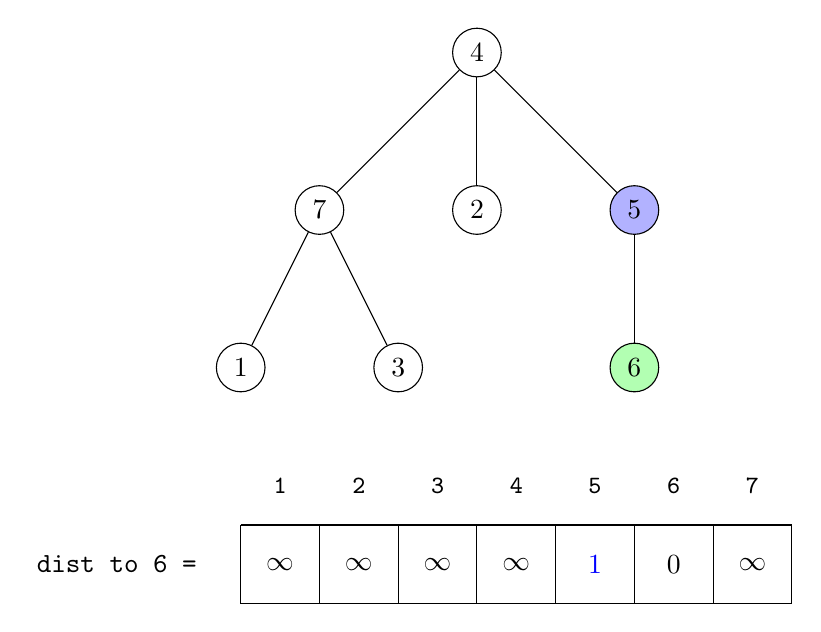
\begin{tikzpicture}

        \begin{scope}
            %\node[opacity=0] (X) at (-1, 0) { $1$ };

            \node[fill=white!30,circle,draw] (D) at (4, 5) { $4$ };
            \node[circle,draw,fill=white!30] (C) at (2, 3) { $7$ };
            \node[circle,draw,fill=white!30] (E) at (4, 3) { $2$ };
            \node[circle,draw,fill=blue!30] (F) at (6, 3) { $5$ };
            \node[circle,draw,fill=white!30] (A) at (1, 1) { $1$ };
            \node[circle,draw,fill=white!30] (B) at (3, 1) { $3$ };
            \node[circle,draw,fill=green!30] (G) at (6, 1) { $6$ };

            \draw (A) -- (C);
            \draw (B) -- (C);
            \draw (C) -- (D);
            \draw (D) -- (E);
            \draw (D) -- (F);
            \draw (F) -- (G);

            \node[anchor=east] at (0.75, -1.5) { \texttt{dist to 6 = } };
            \draw (1, -2) grid (8, -1);

            \node at (1.5, -0.5) { \small \texttt{1} };
            \node at (2.5, -0.5) { \small \texttt{2} };
            \node at (3.5, -0.5) { \small \texttt{3} };
            \node at (4.5, -0.5) { \small \texttt{4} };
            \node at (5.5, -0.5) { \small \texttt{5} };
            \node at (6.5, -0.5) { \small \texttt{6} };
            \node at (7.5, -0.5) { \small \texttt{7} };

            \node at (1.5, -1.5) { \textcolor{black}{$\infty$} };
            \node at (2.5, -1.5) { \textcolor{black}{$\infty$} };
            \node at (3.5, -1.5) { \textcolor{black}{$\infty$} };
            \node at (4.5, -1.5) { \textcolor{black}{$\infty$} };
            \node at (5.5, -1.5) { \textcolor{blue}{$1$} };
            \node at (6.5, -1.5) { \textcolor{black}{$0$} };
            \node at (7.5, -1.5) { \textcolor{black}{$\infty$} };
        \end{scope}
    \end{tikzpicture}

\end{frame}

\begin{frame}[fragile]{Visualização do algoritmo que computa o diâmetro com DFS}

    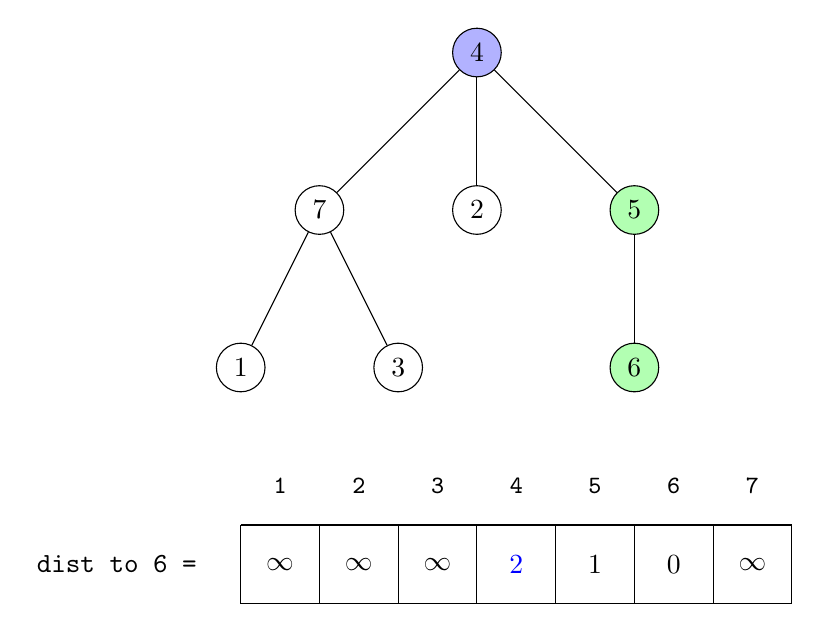
\begin{tikzpicture}

        \begin{scope}
            %\node[opacity=0] (X) at (-1, 0) { $1$ };

            \node[fill=blue!30,circle,draw] (D) at (4, 5) { $4$ };
            \node[circle,draw,fill=white!30] (C) at (2, 3) { $7$ };
            \node[circle,draw,fill=white!30] (E) at (4, 3) { $2$ };
            \node[circle,draw,fill=green!30] (F) at (6, 3) { $5$ };
            \node[circle,draw,fill=white!30] (A) at (1, 1) { $1$ };
            \node[circle,draw,fill=white!30] (B) at (3, 1) { $3$ };
            \node[circle,draw,fill=green!30] (G) at (6, 1) { $6$ };

            \draw (A) -- (C);
            \draw (B) -- (C);
            \draw (C) -- (D);
            \draw (D) -- (E);
            \draw (D) -- (F);
            \draw (F) -- (G);

            \node[anchor=east] at (0.75, -1.5) { \texttt{dist to 6 = } };
            \draw (1, -2) grid (8, -1);

            \node at (1.5, -0.5) { \small \texttt{1} };
            \node at (2.5, -0.5) { \small \texttt{2} };
            \node at (3.5, -0.5) { \small \texttt{3} };
            \node at (4.5, -0.5) { \small \texttt{4} };
            \node at (5.5, -0.5) { \small \texttt{5} };
            \node at (6.5, -0.5) { \small \texttt{6} };
            \node at (7.5, -0.5) { \small \texttt{7} };

            \node at (1.5, -1.5) { \textcolor{black}{$\infty$} };
            \node at (2.5, -1.5) { \textcolor{black}{$\infty$} };
            \node at (3.5, -1.5) { \textcolor{black}{$\infty$} };
            \node at (4.5, -1.5) { \textcolor{blue}{$2$} };
            \node at (5.5, -1.5) { \textcolor{black}{$1$} };
            \node at (6.5, -1.5) { \textcolor{black}{$0$} };
            \node at (7.5, -1.5) { \textcolor{black}{$\infty$} };
        \end{scope}
    \end{tikzpicture}

\end{frame}


\begin{frame}[fragile]{Visualização do algoritmo que computa o diâmetro com DFS}

    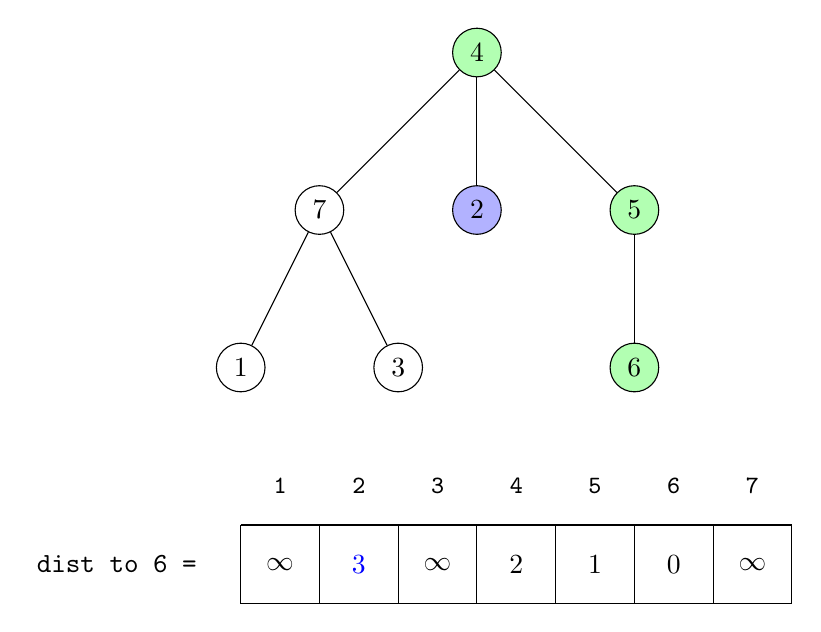
\begin{tikzpicture}

        \begin{scope}
            %\node[opacity=0] (X) at (-1, 0) { $1$ };

            \node[fill=green!30,circle,draw] (D) at (4, 5) { $4$ };
            \node[circle,draw,fill=white!30] (C) at (2, 3) { $7$ };
            \node[circle,draw,fill=blue!30] (E) at (4, 3) { $2$ };
            \node[circle,draw,fill=green!30] (F) at (6, 3) { $5$ };
            \node[circle,draw,fill=white!30] (A) at (1, 1) { $1$ };
            \node[circle,draw,fill=white!30] (B) at (3, 1) { $3$ };
            \node[circle,draw,fill=green!30] (G) at (6, 1) { $6$ };

            \draw (A) -- (C);
            \draw (B) -- (C);
            \draw (C) -- (D);
            \draw (D) -- (E);
            \draw (D) -- (F);
            \draw (F) -- (G);

            \node[anchor=east] at (0.75, -1.5) { \texttt{dist to 6 = } };
            \draw (1, -2) grid (8, -1);

            \node at (1.5, -0.5) { \small \texttt{1} };
            \node at (2.5, -0.5) { \small \texttt{2} };
            \node at (3.5, -0.5) { \small \texttt{3} };
            \node at (4.5, -0.5) { \small \texttt{4} };
            \node at (5.5, -0.5) { \small \texttt{5} };
            \node at (6.5, -0.5) { \small \texttt{6} };
            \node at (7.5, -0.5) { \small \texttt{7} };

            \node at (1.5, -1.5) { \textcolor{black}{$\infty$} };
            \node at (2.5, -1.5) { \textcolor{blue}{$3$} };
            \node at (3.5, -1.5) { \textcolor{black}{$\infty$} };
            \node at (4.5, -1.5) { \textcolor{black}{$2$} };
            \node at (5.5, -1.5) { \textcolor{black}{$1$} };
            \node at (6.5, -1.5) { \textcolor{black}{$0$} };
            \node at (7.5, -1.5) { \textcolor{black}{$\infty$} };
        \end{scope}
    \end{tikzpicture}

\end{frame}

\begin{frame}[fragile]{Visualização do algoritmo que computa o diâmetro com DFS}

    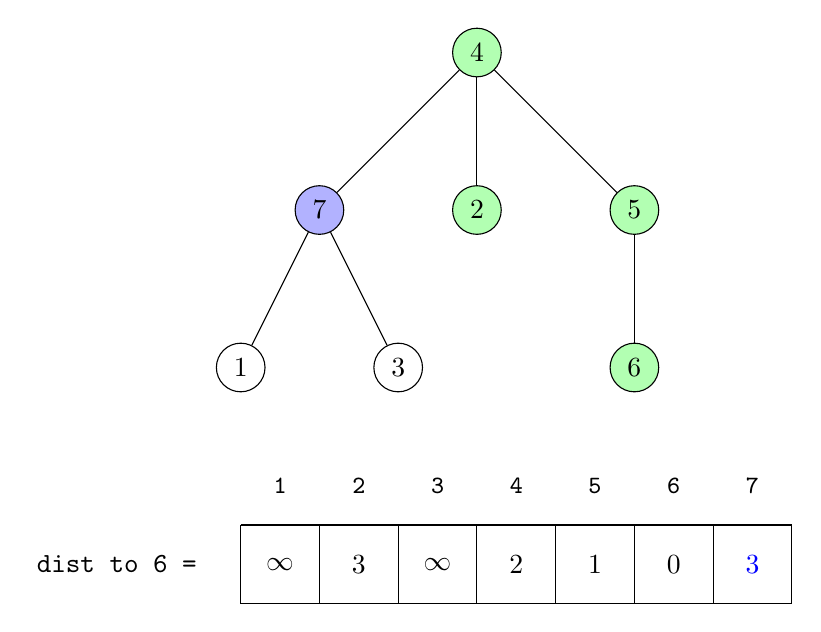
\begin{tikzpicture}

        \begin{scope}
            %\node[opacity=0] (X) at (-1, 0) { $1$ };

            \node[fill=green!30,circle,draw] (D) at (4, 5) { $4$ };
            \node[circle,draw,fill=blue!30] (C) at (2, 3) { $7$ };
            \node[circle,draw,fill=green!30] (E) at (4, 3) { $2$ };
            \node[circle,draw,fill=green!30] (F) at (6, 3) { $5$ };
            \node[circle,draw,fill=white!30] (A) at (1, 1) { $1$ };
            \node[circle,draw,fill=white!30] (B) at (3, 1) { $3$ };
            \node[circle,draw,fill=green!30] (G) at (6, 1) { $6$ };

            \draw (A) -- (C);
            \draw (B) -- (C);
            \draw (C) -- (D);
            \draw (D) -- (E);
            \draw (D) -- (F);
            \draw (F) -- (G);

            \node[anchor=east] at (0.75, -1.5) { \texttt{dist to 6 = } };
            \draw (1, -2) grid (8, -1);

            \node at (1.5, -0.5) { \small \texttt{1} };
            \node at (2.5, -0.5) { \small \texttt{2} };
            \node at (3.5, -0.5) { \small \texttt{3} };
            \node at (4.5, -0.5) { \small \texttt{4} };
            \node at (5.5, -0.5) { \small \texttt{5} };
            \node at (6.5, -0.5) { \small \texttt{6} };
            \node at (7.5, -0.5) { \small \texttt{7} };

            \node at (1.5, -1.5) { \textcolor{black}{$\infty$} };
            \node at (2.5, -1.5) { \textcolor{black}{$3$} };
            \node at (3.5, -1.5) { \textcolor{black}{$\infty$} };
            \node at (4.5, -1.5) { \textcolor{black}{$2$} };
            \node at (5.5, -1.5) { \textcolor{black}{$1$} };
            \node at (6.5, -1.5) { \textcolor{black}{$0$} };
            \node at (7.5, -1.5) { \textcolor{blue}{$3$} };
        \end{scope}
    \end{tikzpicture}

\end{frame}

\begin{frame}[fragile]{Visualização do algoritmo que computa o diâmetro com DFS}

    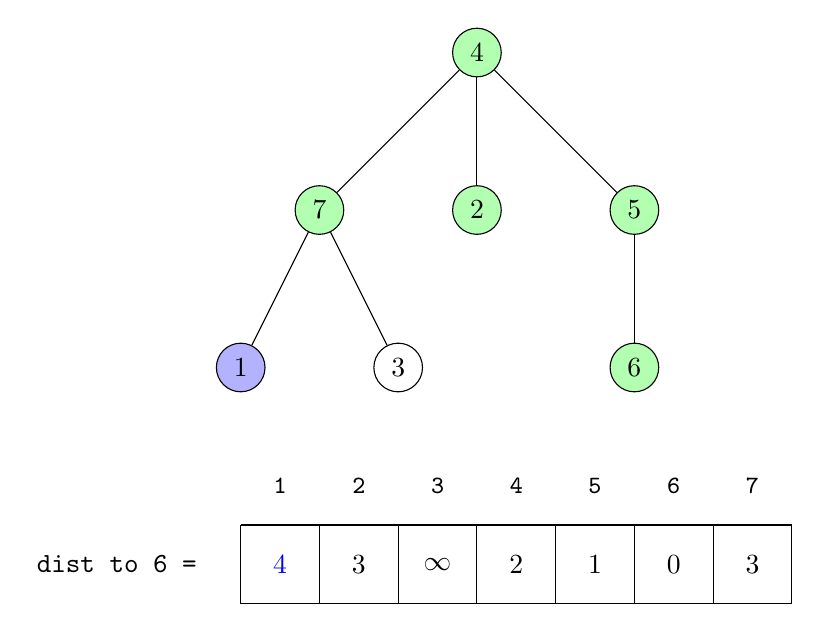
\begin{tikzpicture}

        \begin{scope}
            %\node[opacity=0] (X) at (-1, 0) { $1$ };

            \node[fill=green!30,circle,draw] (D) at (4, 5) { $4$ };
            \node[circle,draw,fill=green!30] (C) at (2, 3) { $7$ };
            \node[circle,draw,fill=green!30] (E) at (4, 3) { $2$ };
            \node[circle,draw,fill=green!30] (F) at (6, 3) { $5$ };
            \node[circle,draw,fill=blue!30] (A) at (1, 1) { $1$ };
            \node[circle,draw,fill=white!30] (B) at (3, 1) { $3$ };
            \node[circle,draw,fill=green!30] (G) at (6, 1) { $6$ };

            \draw (A) -- (C);
            \draw (B) -- (C);
            \draw (C) -- (D);
            \draw (D) -- (E);
            \draw (D) -- (F);
            \draw (F) -- (G);

            \node[anchor=east] at (0.75, -1.5) { \texttt{dist to 6 = } };
            \draw (1, -2) grid (8, -1);

            \node at (1.5, -0.5) { \small \texttt{1} };
            \node at (2.5, -0.5) { \small \texttt{2} };
            \node at (3.5, -0.5) { \small \texttt{3} };
            \node at (4.5, -0.5) { \small \texttt{4} };
            \node at (5.5, -0.5) { \small \texttt{5} };
            \node at (6.5, -0.5) { \small \texttt{6} };
            \node at (7.5, -0.5) { \small \texttt{7} };

            \node at (1.5, -1.5) { \textcolor{blue}{$4$} };
            \node at (2.5, -1.5) { \textcolor{black}{$3$} };
            \node at (3.5, -1.5) { \textcolor{black}{$\infty$} };
            \node at (4.5, -1.5) { \textcolor{black}{$2$} };
            \node at (5.5, -1.5) { \textcolor{black}{$1$} };
            \node at (6.5, -1.5) { \textcolor{black}{$0$} };
            \node at (7.5, -1.5) { \textcolor{black}{$3$} };
        \end{scope}
    \end{tikzpicture}

\end{frame}

\begin{frame}[fragile]{Visualização do algoritmo que computa o diâmetro com DFS}

    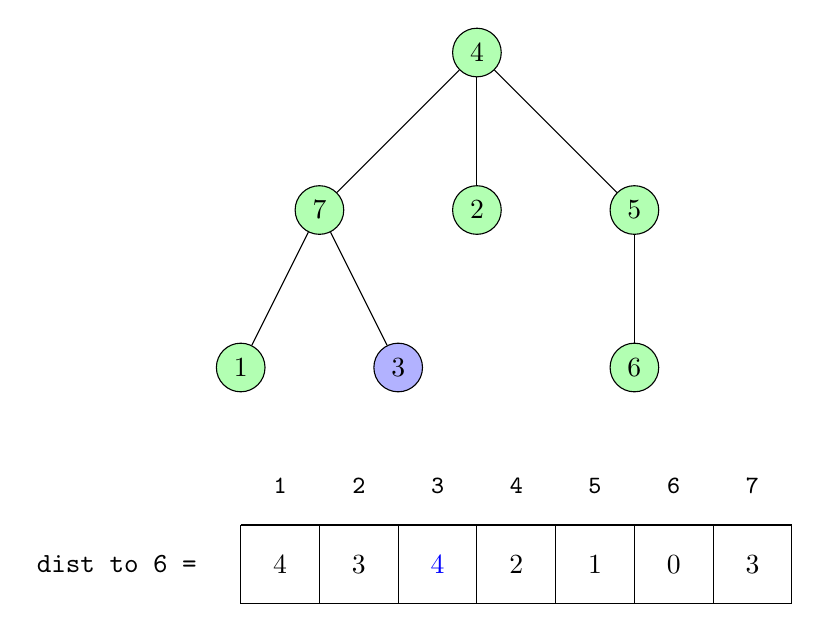
\begin{tikzpicture}

        \begin{scope}
            %\node[opacity=0] (X) at (-1, 0) { $1$ };

            \node[fill=green!30,circle,draw] (D) at (4, 5) { $4$ };
            \node[circle,draw,fill=green!30] (C) at (2, 3) { $7$ };
            \node[circle,draw,fill=green!30] (E) at (4, 3) { $2$ };
            \node[circle,draw,fill=green!30] (F) at (6, 3) { $5$ };
            \node[circle,draw,fill=green!30] (A) at (1, 1) { $1$ };
            \node[circle,draw,fill=blue!30] (B) at (3, 1) { $3$ };
            \node[circle,draw,fill=green!30] (G) at (6, 1) { $6$ };

            \draw (A) -- (C);
            \draw (B) -- (C);
            \draw (C) -- (D);
            \draw (D) -- (E);
            \draw (D) -- (F);
            \draw (F) -- (G);

            \node[anchor=east] at (0.75, -1.5) { \texttt{dist to 6 = } };
            \draw (1, -2) grid (8, -1);

            \node at (1.5, -0.5) { \small \texttt{1} };
            \node at (2.5, -0.5) { \small \texttt{2} };
            \node at (3.5, -0.5) { \small \texttt{3} };
            \node at (4.5, -0.5) { \small \texttt{4} };
            \node at (5.5, -0.5) { \small \texttt{5} };
            \node at (6.5, -0.5) { \small \texttt{6} };
            \node at (7.5, -0.5) { \small \texttt{7} };

            \node at (1.5, -1.5) { \textcolor{black}{$4$} };
            \node at (2.5, -1.5) { \textcolor{black}{$3$} };
            \node at (3.5, -1.5) { \textcolor{blue}{$4$} };
            \node at (4.5, -1.5) { \textcolor{black}{$2$} };
            \node at (5.5, -1.5) { \textcolor{black}{$1$} };
            \node at (6.5, -1.5) { \textcolor{black}{$0$} };
            \node at (7.5, -1.5) { \textcolor{black}{$3$} };
        \end{scope}
    \end{tikzpicture}

\end{frame}

\begin{frame}[fragile]{Implementação da rotina que computa o diâmetro com DFS}
    \inputsnippet{c++}{1}{21}{diameter.cpp}
\end{frame}

\begin{frame}[fragile]{Implementação da rotina que computa o diâmetro com DFS}
    \inputsnippet{c++}{22}{39}{diameter.cpp}
\end{frame}

\begin{frame}[fragile]{Implementação da rotina que computa o diâmetro com DFS}
    \inputsnippet{c++}{40}{60}{diameter.cpp}
\end{frame}

